\chapter{Results and Discussion\label{cha:chapter6}}

This chapter describes the results obtained from the above two schemes. The quantities used below in this section are dimensionless unless specified. 
We have considered pure Aluminum as a crystalline material with sharp melting point and SS304L as an amorphous material which melts over a range of temperature. The properties of Al are summarized in the table \ref{table:AL}\cite{verhoeven2003modelling} and the properties of SS304 are summarized in the table \ref{table:SS304L}\cite{Zhou_2006}. 
\begin{table}[htbp]
    \centering
    \renewcommand{\arraystretch}{1.5} % Increase the row height by 1.5 times
    \begin{tabular}{|c|c|}
        \hline
         Property & Value \\
         \hline
         Thermal conductivity $k$ & $2.3 \ \text{x}\ 10^2\, \frac{W}{mK}$\\
         \hline
         Density $\rho$ & $2.7\ \text{x} \ 10^3\, \frac{kg}{m^3}$\\
         \hline
         Melting temperature $T_m$ & $9.3\ \text{x} \ 10^2 K$\\
         \hline
         Vapour temperature $T_v$ & $2.5 \ \text{x} \ 10^3 K$\\
         \hline
         Specific heat of the solid c & $9.0 \ \text{x} \ 10^2 \frac{J}{kg K}$\\
         \hline
         Latent heat of fusion $L_f$ & $3.6 \ \text{x} \ 10^5 \frac{J}{kg}$\\
         \hline
    \end{tabular}
    \caption{Properties of Al}
    \label{table:AL}
\end{table}\\

\begin{table}[htbp]
    \centering
    \renewcommand{\arraystretch}{1.5} % Increase the row height by 1.5 times
    \begin{tabular}{|c|c|}
        \hline
         Property & Value \\
         \hline
         Thermal conductivity $k$ & $22\, \frac{W}{mK}$\\
         \hline
         Density $\rho$ & $7.2\ \text{x} \ 10^3\, \frac{kg}{m^3}$\\
         \hline
         Solidus temperature $T_{sol}$ & $16.7\ \text{x} \ 10^2 K$\\
         \hline
         Liquidus temperature $T_{sol}$ & $17.27\ \text{x} \ 10^2 K$\\
         \hline
         Vapour temperature $T_v$ & $3.375 \ \text{x} \ 10^3 K$\\
         \hline
         Specific heat of the solid c & $7.0 \ \text{x} \ 10^2 \frac{J}{kg K}$\\
         \hline
         Latent heat of fusion $L_f$ & $2.47 \ \text{x} \ 10^5 \frac{J}{kg}$\\
         \hline
    \end{tabular}
    \caption{Properties of SS304}
    \label{table:SS304L}
\end{table}
Further more we have assumed that the reference laser power $I_{ref}$ is 1.5 x $10^{10} \frac{W}{m^2}$.
\section{The Enthalpy Problem\label{sec:env}}
The results of the enthalpy problem are discussed below.

\subsection{Verification of Heat Transfer Results with Type I Boundary Conditions}

The figure \ref{fig:Temp_Dist_in_crystal} shows the temperature distribution in Aluminium material obtained by the numerical scheme and the analytical scheme along with the initial temperature distribution. We considered 150 elements and $\Delta t$ was assumed to be 0.0001 with input laser power I = 1.5 x $10^{10} \ \frac{W}{m^2}$. The end time for this simulation was set to 0.2. The root mean square error for Al using these settings was found to be 0.092. Further, a reduction of error was observed as we decreased the time step $\Delta t$ and is shown in figure \ref{fig:convergence_Al}. 

\begin{figure}[h]
  \centering
  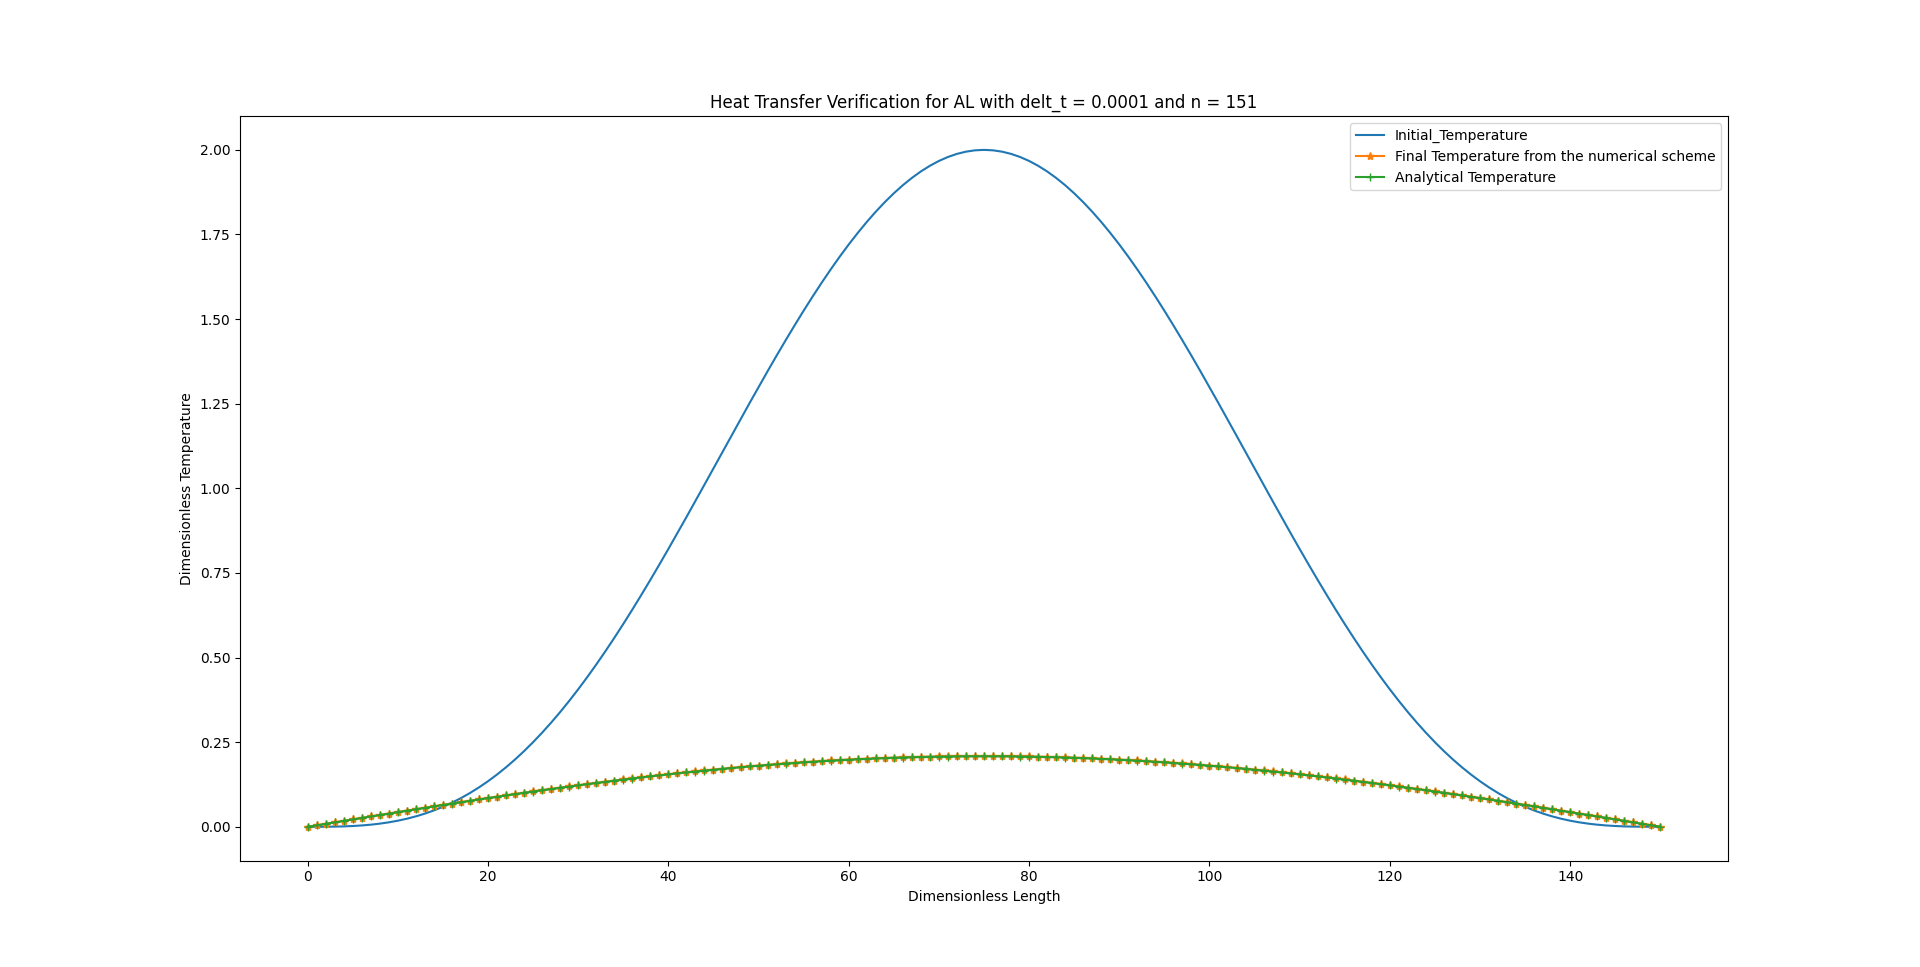
\includegraphics[width=15cm]{img/Al_Type1.png}
  \caption{Verification of the temperature distribution in Al for type I BC}
  \label{fig:Temp_Dist_in_crystal}
\end{figure}

Similarly, the figure \ref{fig:Temp_Dist_in_amorphous} shows the temperature distribution obtained from numerical and the analytical scheme for end time = 0.2 in SS304L for type 1 BC along with the initial temperature distribution. We considered 151 nodes and $\Delta t$ = 0.0001 was assumed. The root mean square error obtained using the above mentioned settings was found to be 0.090.

\begin{figure}[h]
  \centering
  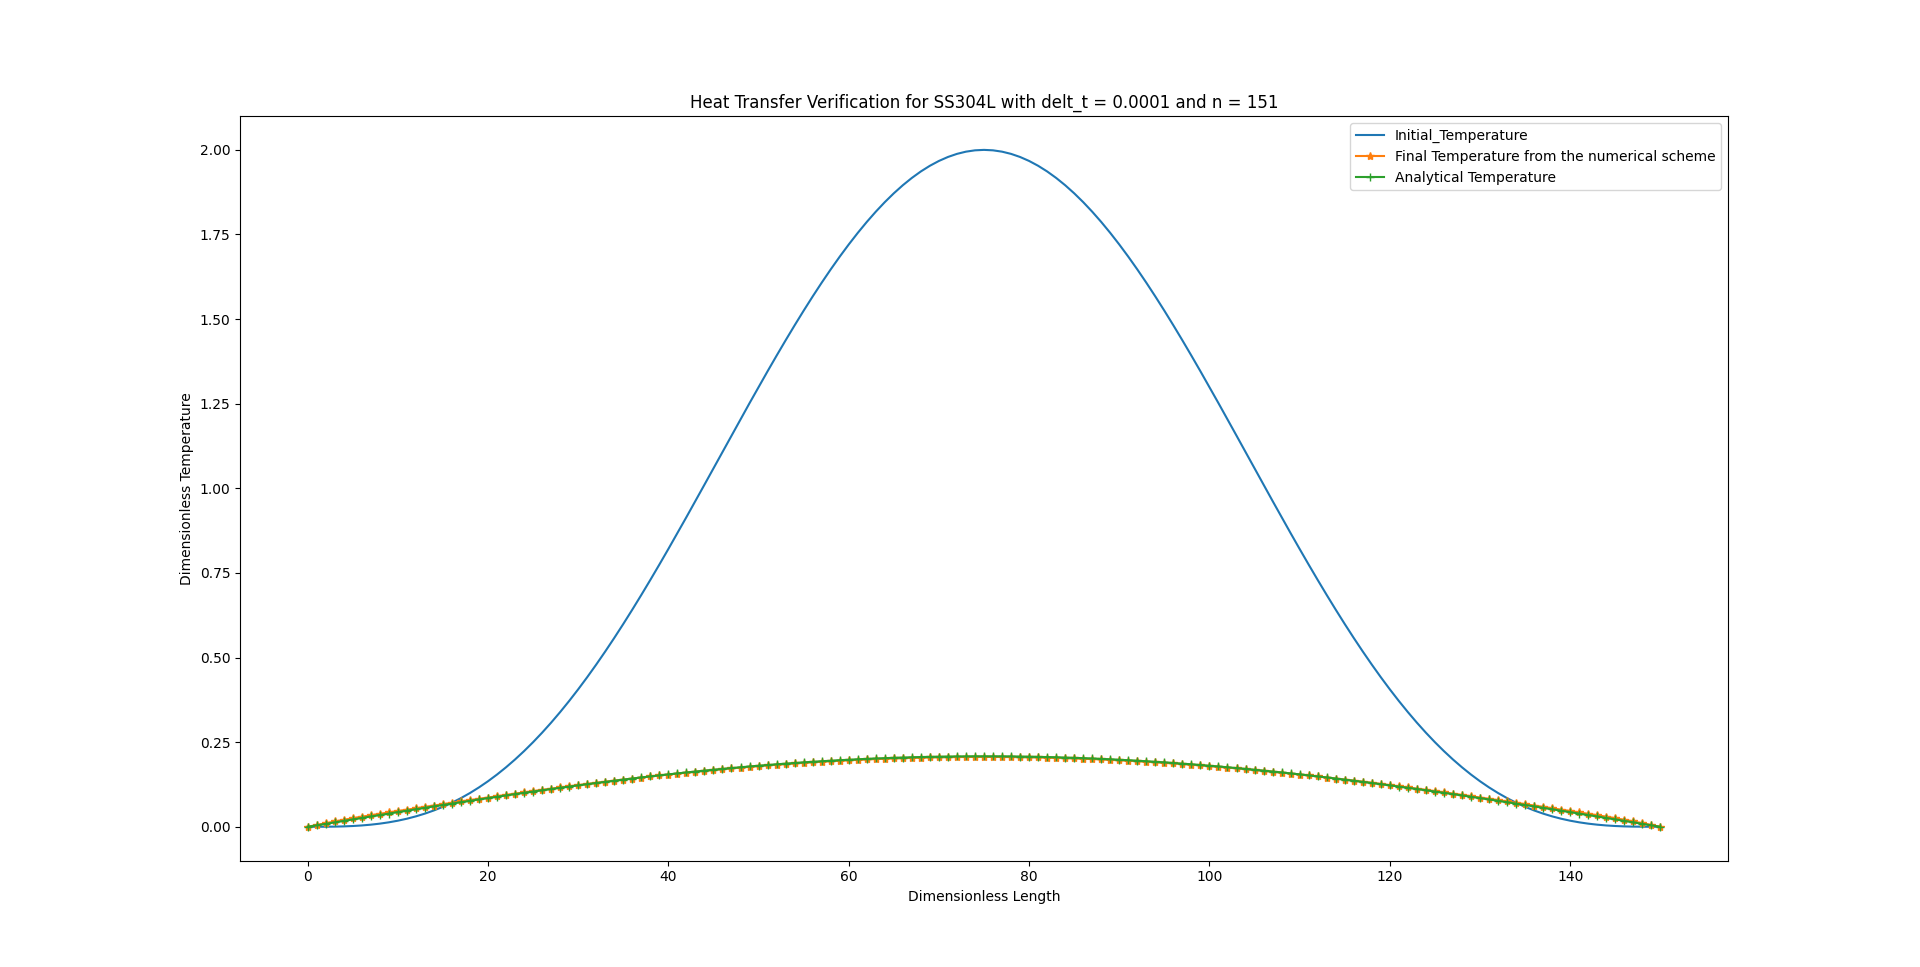
\includegraphics[width=17cm]{img/Amor_t1.png}
  \caption{Verification of the temperature distribution in SS304L for type I BC}
  \label{fig:Temp_Dist_in_amorphous}
\end{figure}
\newpage
To investigate the impact of time step ($\Delta t$) on the convergence of our solution, we conducted four separate runs, each with a different $\Delta t$ value. Throughout all runs, we maintained consistent settings, including a fixed input laser power of $1.5 \times 10^{10} \ \frac{W}{m^2}$, a total of 151 nodes, and a constant end time = 0.2. The only variable we altered was the time step.\\
In the initial run (Run 1), we set $\Delta t$ to 0.1. Subsequently, in Run 2, we reduced $\Delta t$ to 0.01. In Run 3, $\Delta t$ was further decreased to 0.001. Finally, in Run 4, we employed a much smaller $\Delta t$ of 0.0001.\\
The x-axis in our results in the figure \ref{fig:convergence_Al} represents the run count, corresponding to the specific $\Delta t$ used in each simulation run.
\begin{figure}[h]
  \centering
  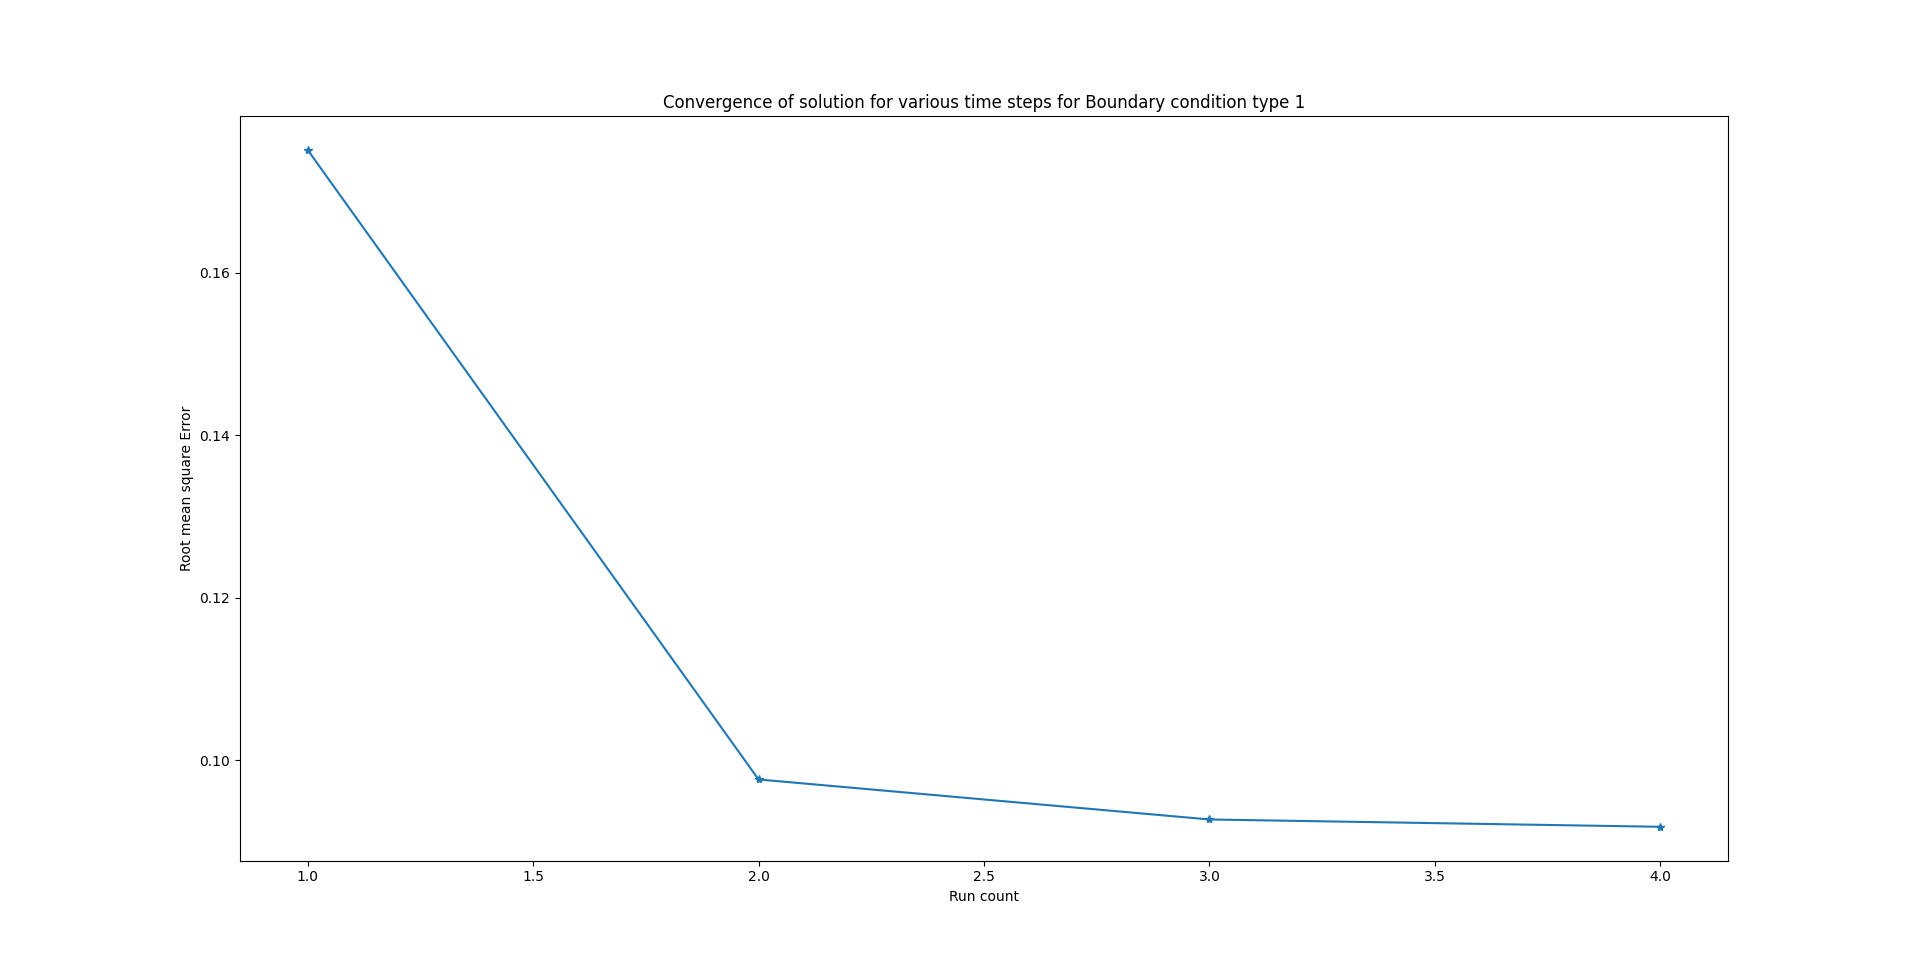
\includegraphics[width=13cm]{img/Error_convergence_for_BS1_delt_time.png}
  \caption{Convergence of the solution in Al for type I BC with variable$\Delta t$}
  \label{fig:convergence_Al}
\end{figure}

On a similar note,we conducted an examination of how the number of nodes influences the error. For this investigation, we maintained consistent settings, including a fixed input laser power of $1.5 \times 10^{10} \ \frac{W}{m^2}$, a constant $\Delta t$ of 0.001, and an end time of 0.2.  The only quantity varied was the number of nodes. The Figure \ref{fig:meshconvergence_Al} illustrates the error reduction as the number of nodes decreases. Notably, beyond 360 nodes, the error remains nearly constant.
\begin{figure}[h]
  \centering
  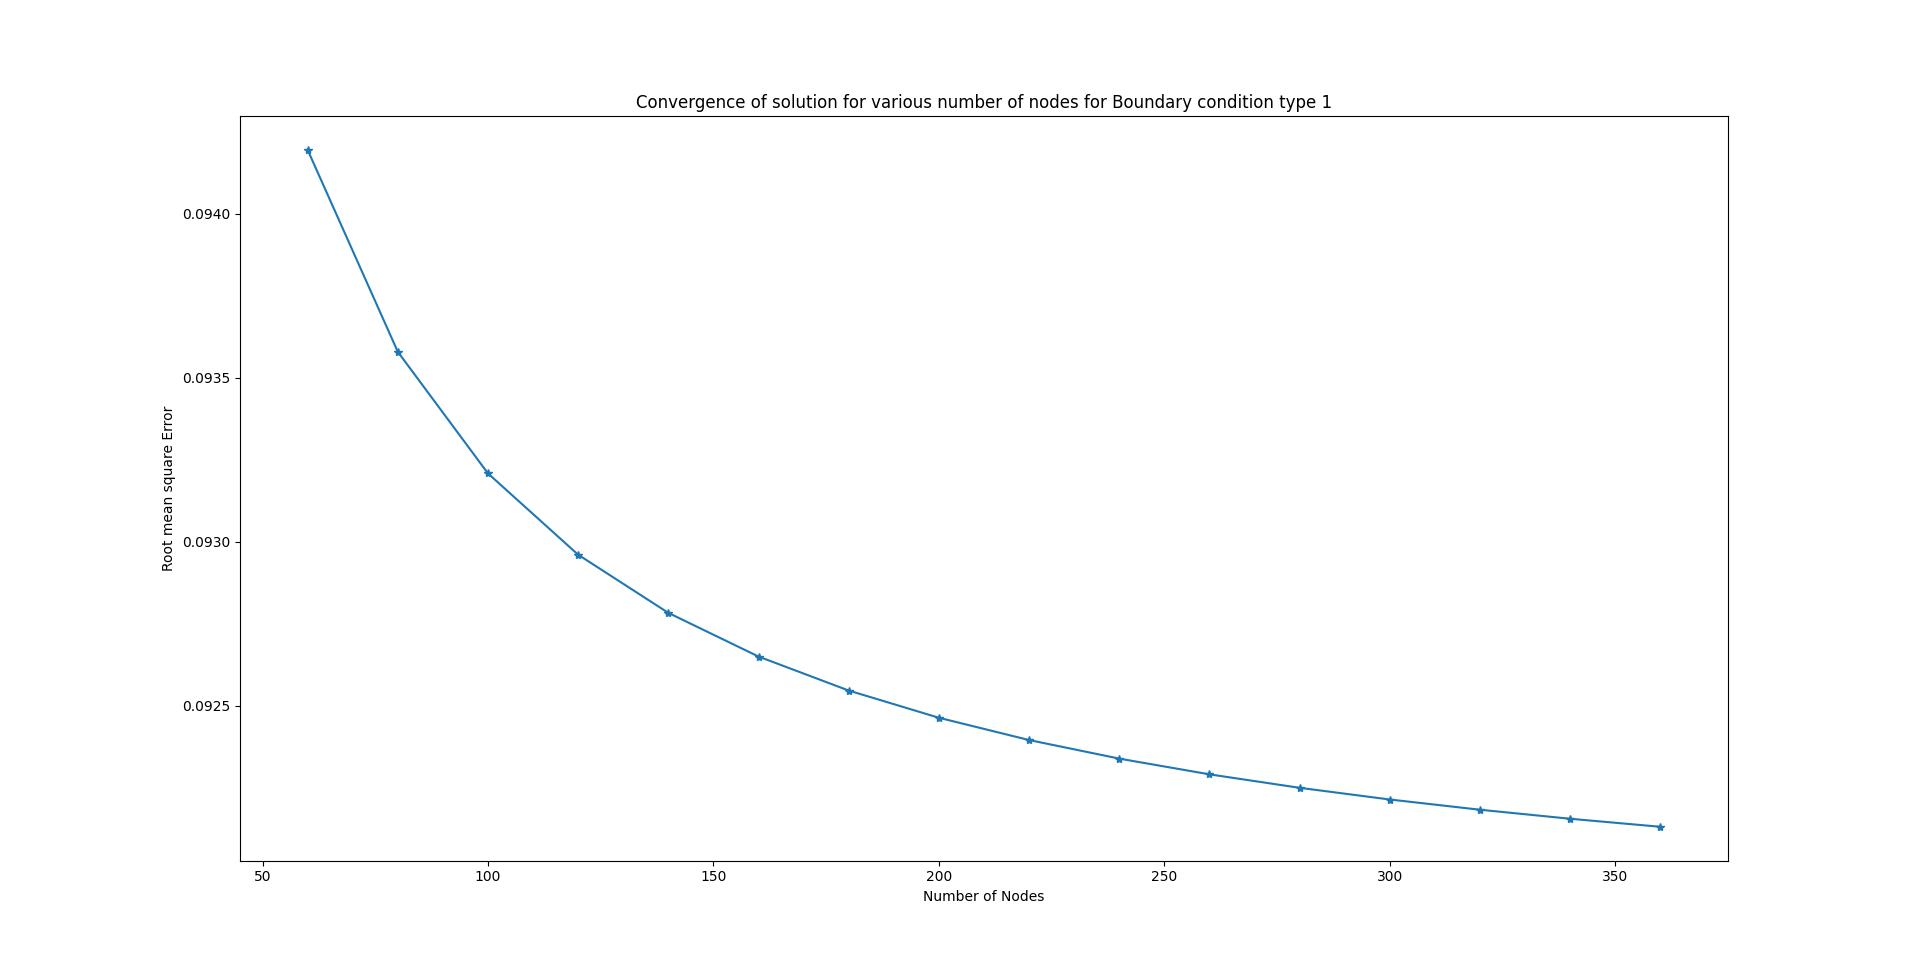
\includegraphics[width=15cm]{img/Nodal_convergence.png}
  \caption{Mesh convergence for Al using type I BC}
  \label{fig:meshconvergence_Al}
\end{figure}
\newpage
\subsection{Verification of Heat Transfer Results with Type II Boundary Conditions}
We may approximate the solution \eqref{eq:Analytical_Solution} by considering only its first term. This approximation is valid when the end time $t$ is greater than $\frac{4}{\pi^2}$, as indicated by Hancock\cite{Hancock}. In our case, with an end time of $t = 0.1$, which is less than $\frac{4}{\pi^2}$, we utilized the first 4 terms of equation \eqref{eq:Analytical_Solution}. Our choice was influenced by the observation presented in Figure \ref{fig:meshconvergence_RMS}, where it is evident that the error approaches nearly zero after adding the first 2 terms. However, for enhanced accuracy, we included the first 4 terms in the series. This error was assessed by monitoring the changes in values as new terms were added to the solution.
\begin{figure}[h]
  \centering
  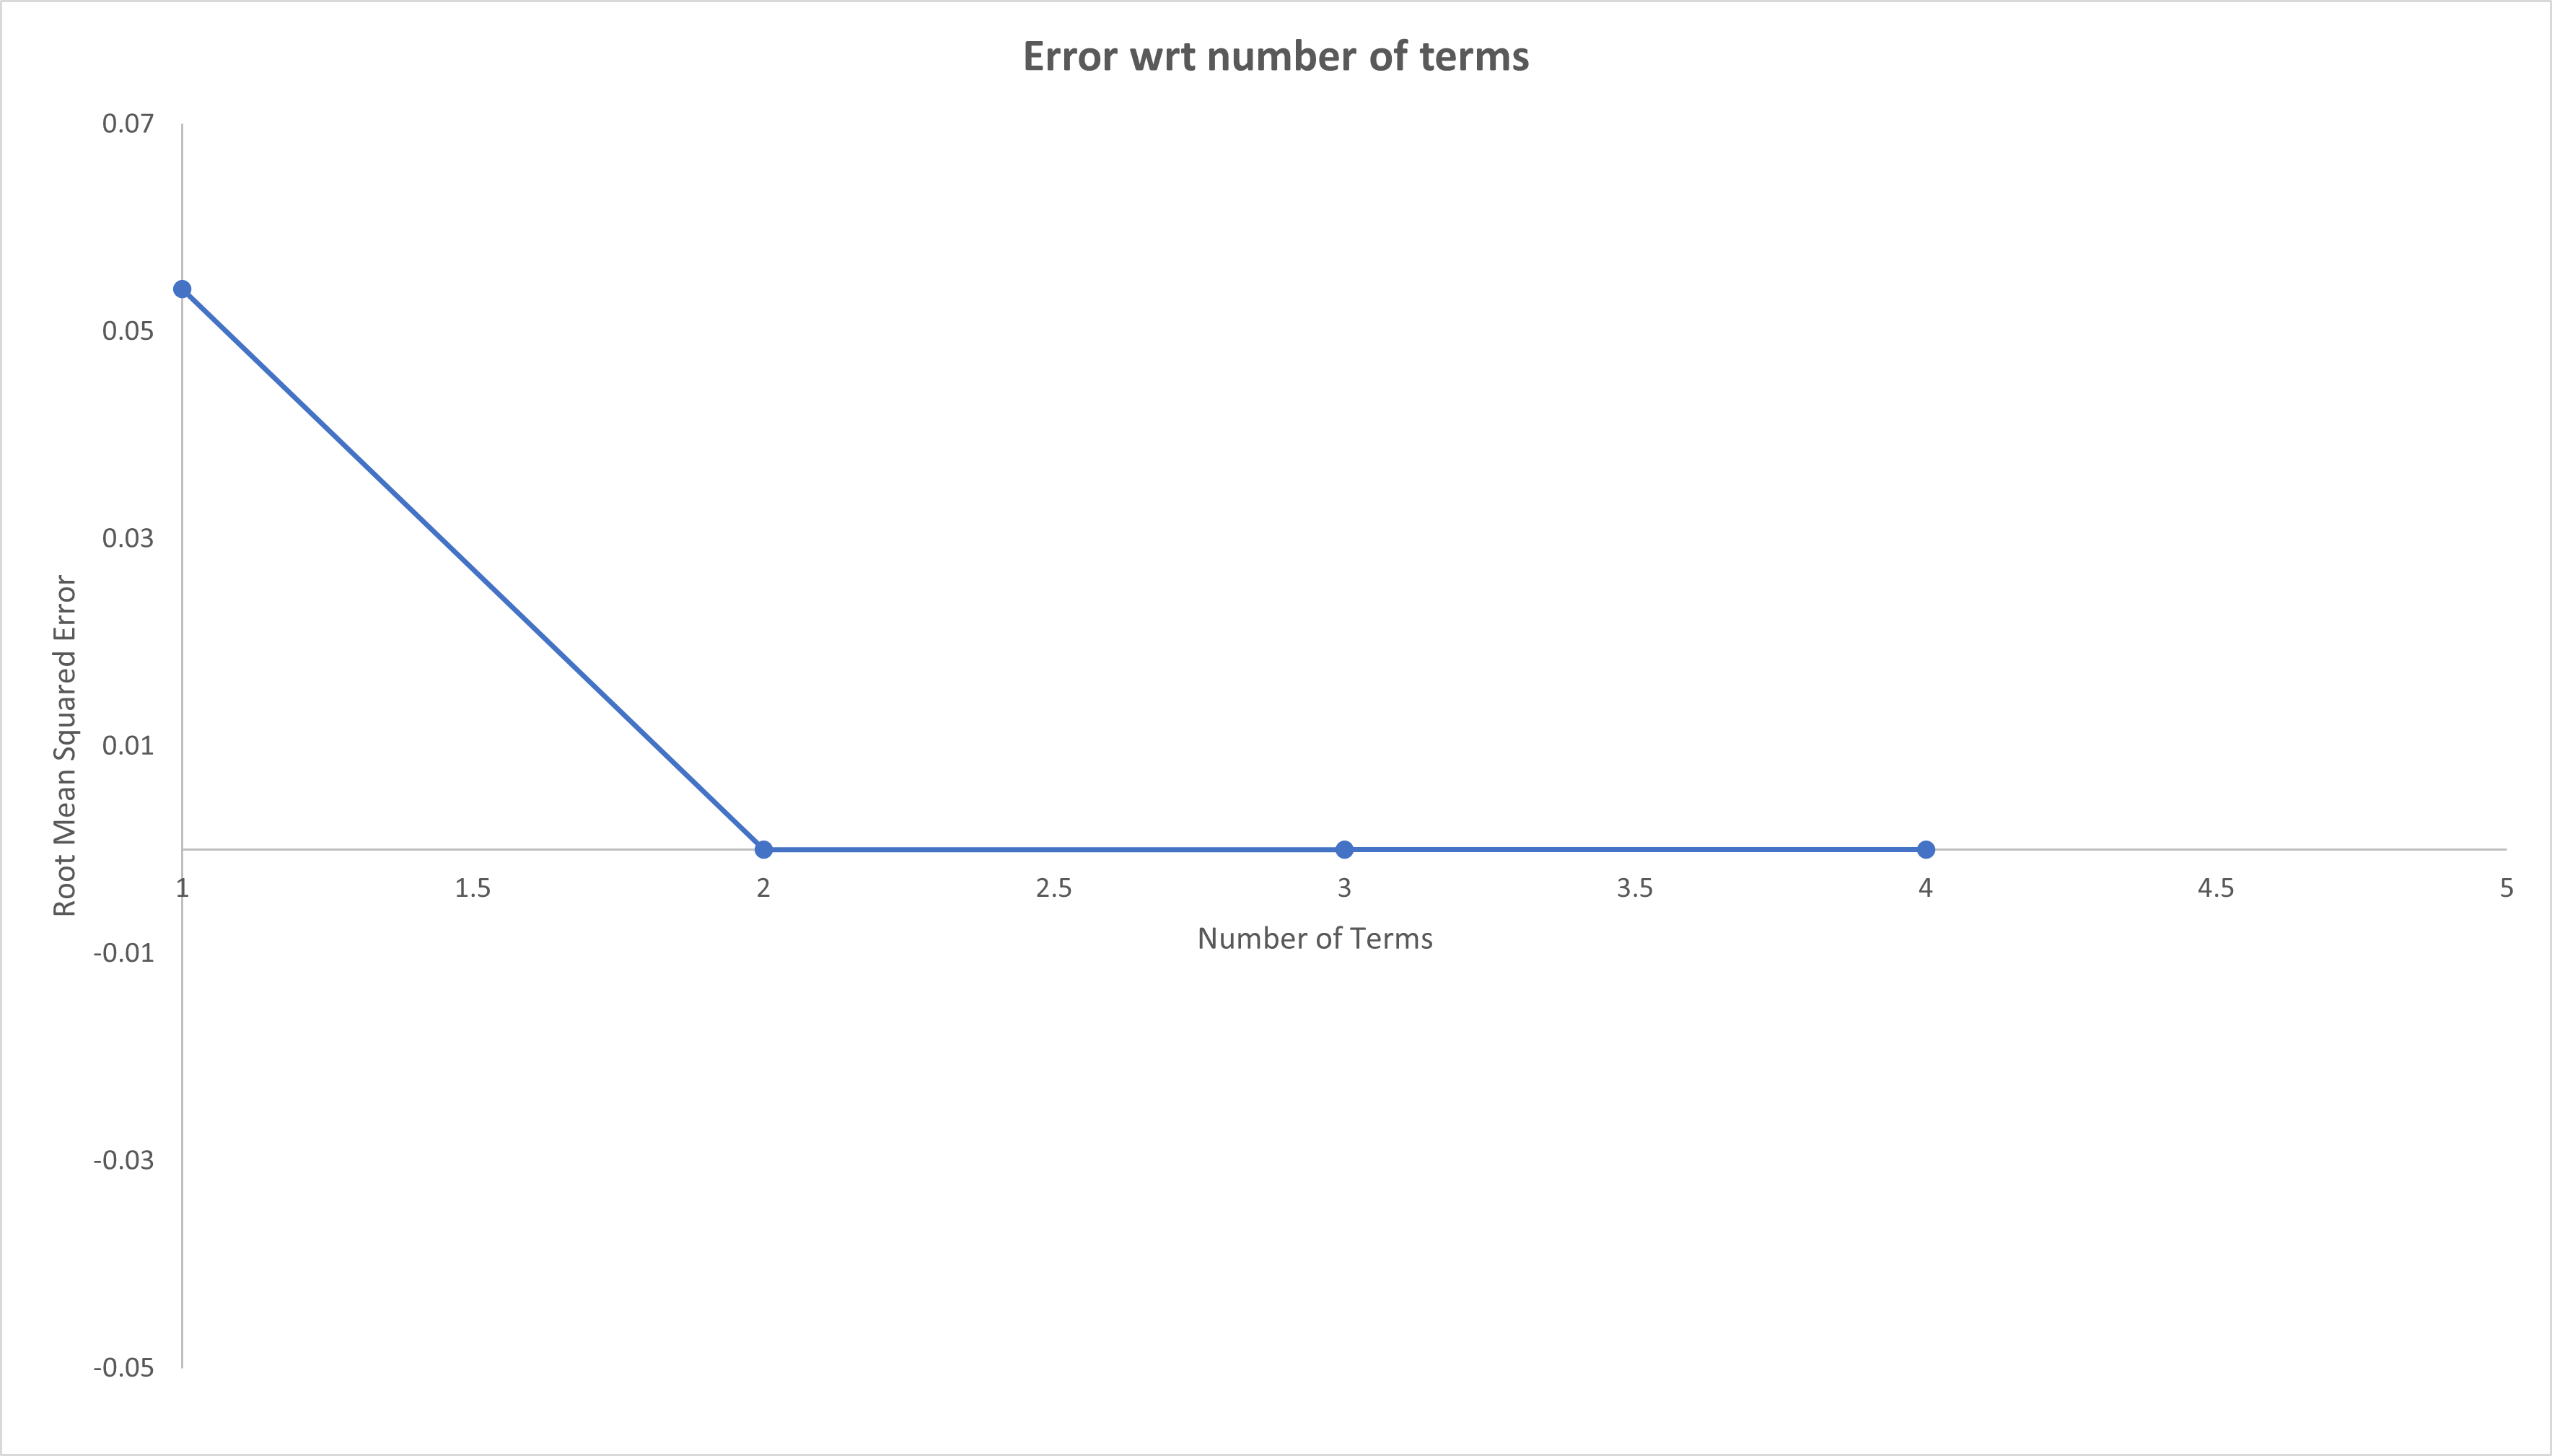
\includegraphics[width=10cm]{img/Error_in_Analytical.png}
  \caption{RMS Error Convergence with Increasing Number of Terms in Series for analytical solution with type II BC.}
  \label{fig:meshconvergence_RMS}
\end{figure}
A similar setting is employed as we used in type I BC, we employ 150 elements and $\Delta t$ was fixed to be 0.0001 with input laser power I = 1.5 x $10^{10} \ \frac{W}{m^2}$. The end time for this simulation was set to 0.1 for both the materials. The figure \ref{fig:Type2} shows the temperature distribution in AL and the figure \ref{fig:Type2SS304L} shows the temperature distribution in SS304L respectively. 
\begin{figure}[h]
  \centering
  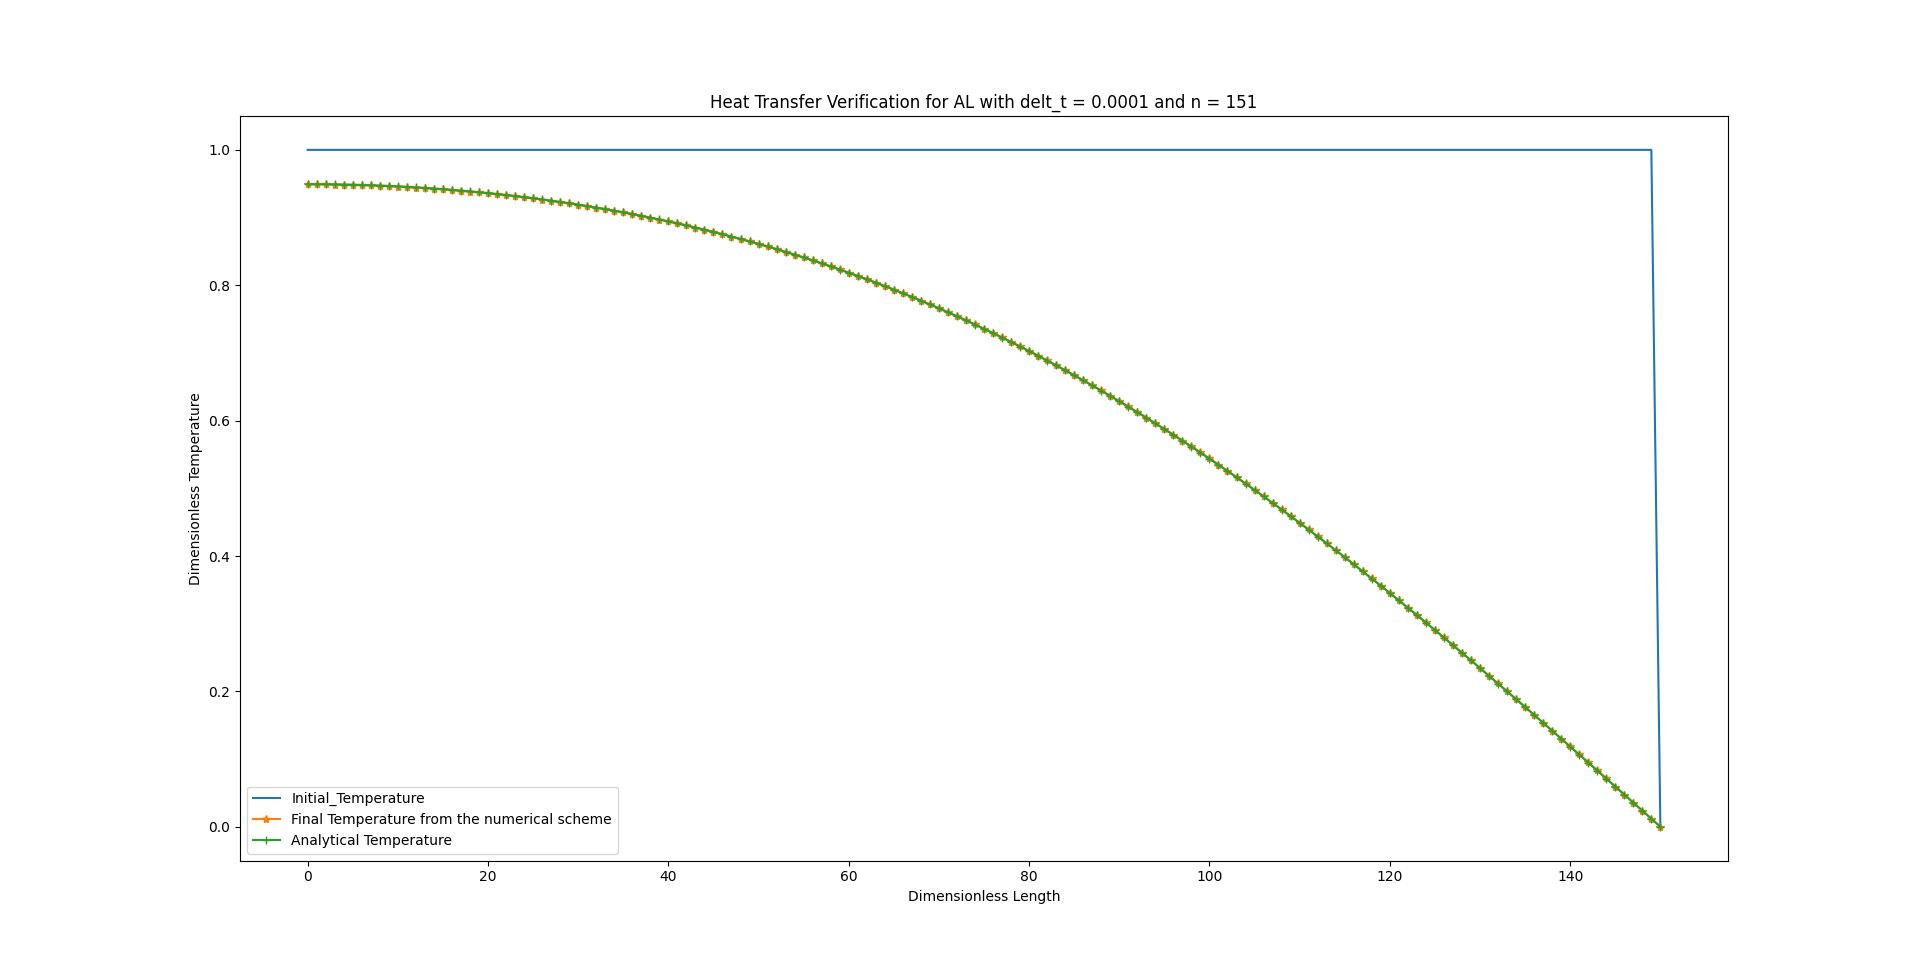
\includegraphics[width=15cm]{img/AL_type2.png}
  \caption{Verification of the temperature distribution in AL for type II BC}
  \label{fig:Type2}
\end{figure}
\begin{figure}[h]
  \centering
  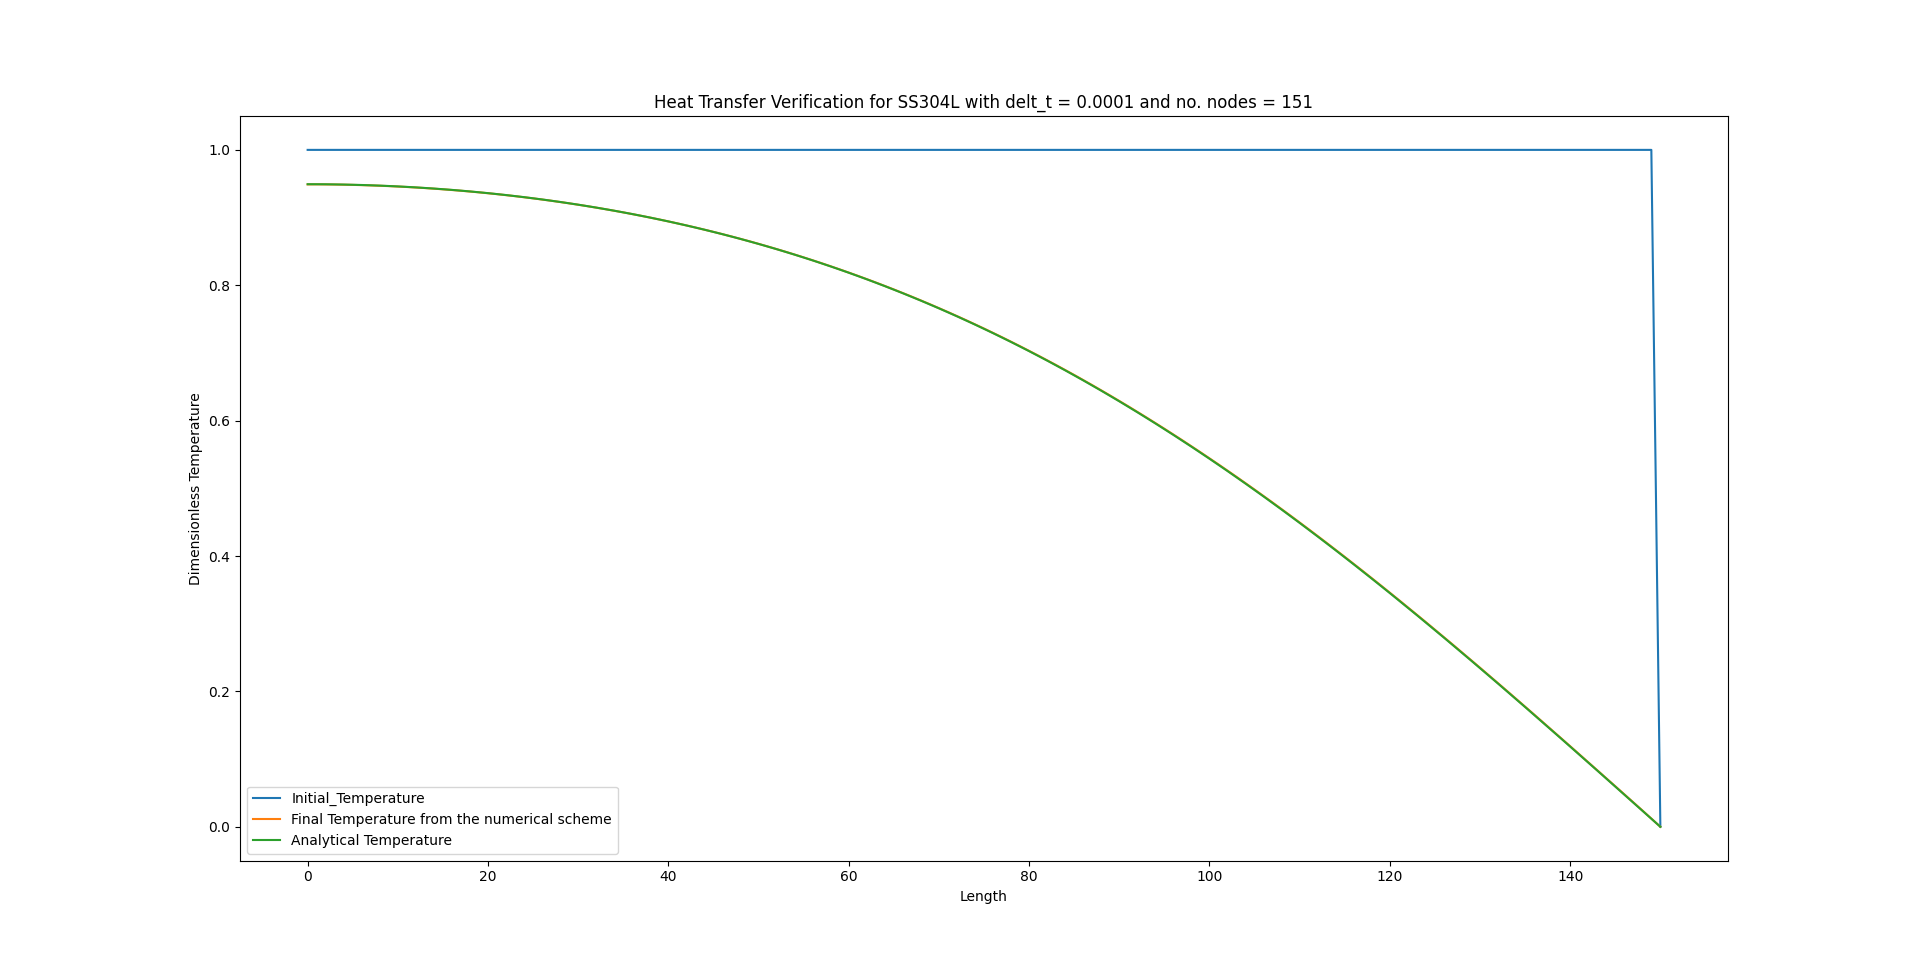
\includegraphics[width=17cm]{img/SS304_T2.png}
  \caption{Verification of the temperature distribution in SS304L for type II BC}
  \label{fig:Type2SS304L}
\end{figure}
\newpage
\subsection{Position of the Phase Change Boundary}
The analytical solution for the phase change boundary without considering the latent heat effects is given by the equation \ref{eq:melt_anal}\cite{verhoeven2003modelling}\cite{pahio(2872)_2015}.
\begin{subequations}
    \begin{align}
        R = \frac{I}{I_{\text{ref}}}\left\{2\sqrt{D}\left(\frac{t}{\pi}^{\frac{1}{2}}\right) \exp\left(-\frac{s^2}{4Dt}\right) - s \operatorname{erfc}\left(\frac{s}{2\sqrt{Dt}}\right)\right\} +T_a = 0 \label{eq:melt_anal}
    \end{align} \label{eq:analytical solution to the position}
\end{subequations}
The position of the phase change boundary is found by Euler Forward Step and Newton Raphson Scheme. For the NRS we need to find the derivative of the equation \ref{eq:melt_anal} with respect to 's'. The equation \ref{eq:derivativemelt_anal} is the derivative of equation \ref{eq:melt_anal} with respect to 's' and was found manually by hand calculations.  
\begin{subequations}
    \begin{align}
       \frac{\partial R}{\partial s} = -\frac{I}{I_{\text{ref}}}\left\{\operatorname{erfc}\left(\frac{s}{2\sqrt{Dt}}\right)\right\} \label{eq:derivativemelt_anal}
    \end{align}
\end{subequations}

Using the equations \ref{eq:melt_anal} and \ref{eq:derivativemelt_anal} we have plotted the analytical solution in figures \ref{fig:phasechange} to \ref{fig:AL_Latenthear} for the verification of the position of the phase front in Al and SS304L for each time step.
\begin{figure}[h]
  \centering
  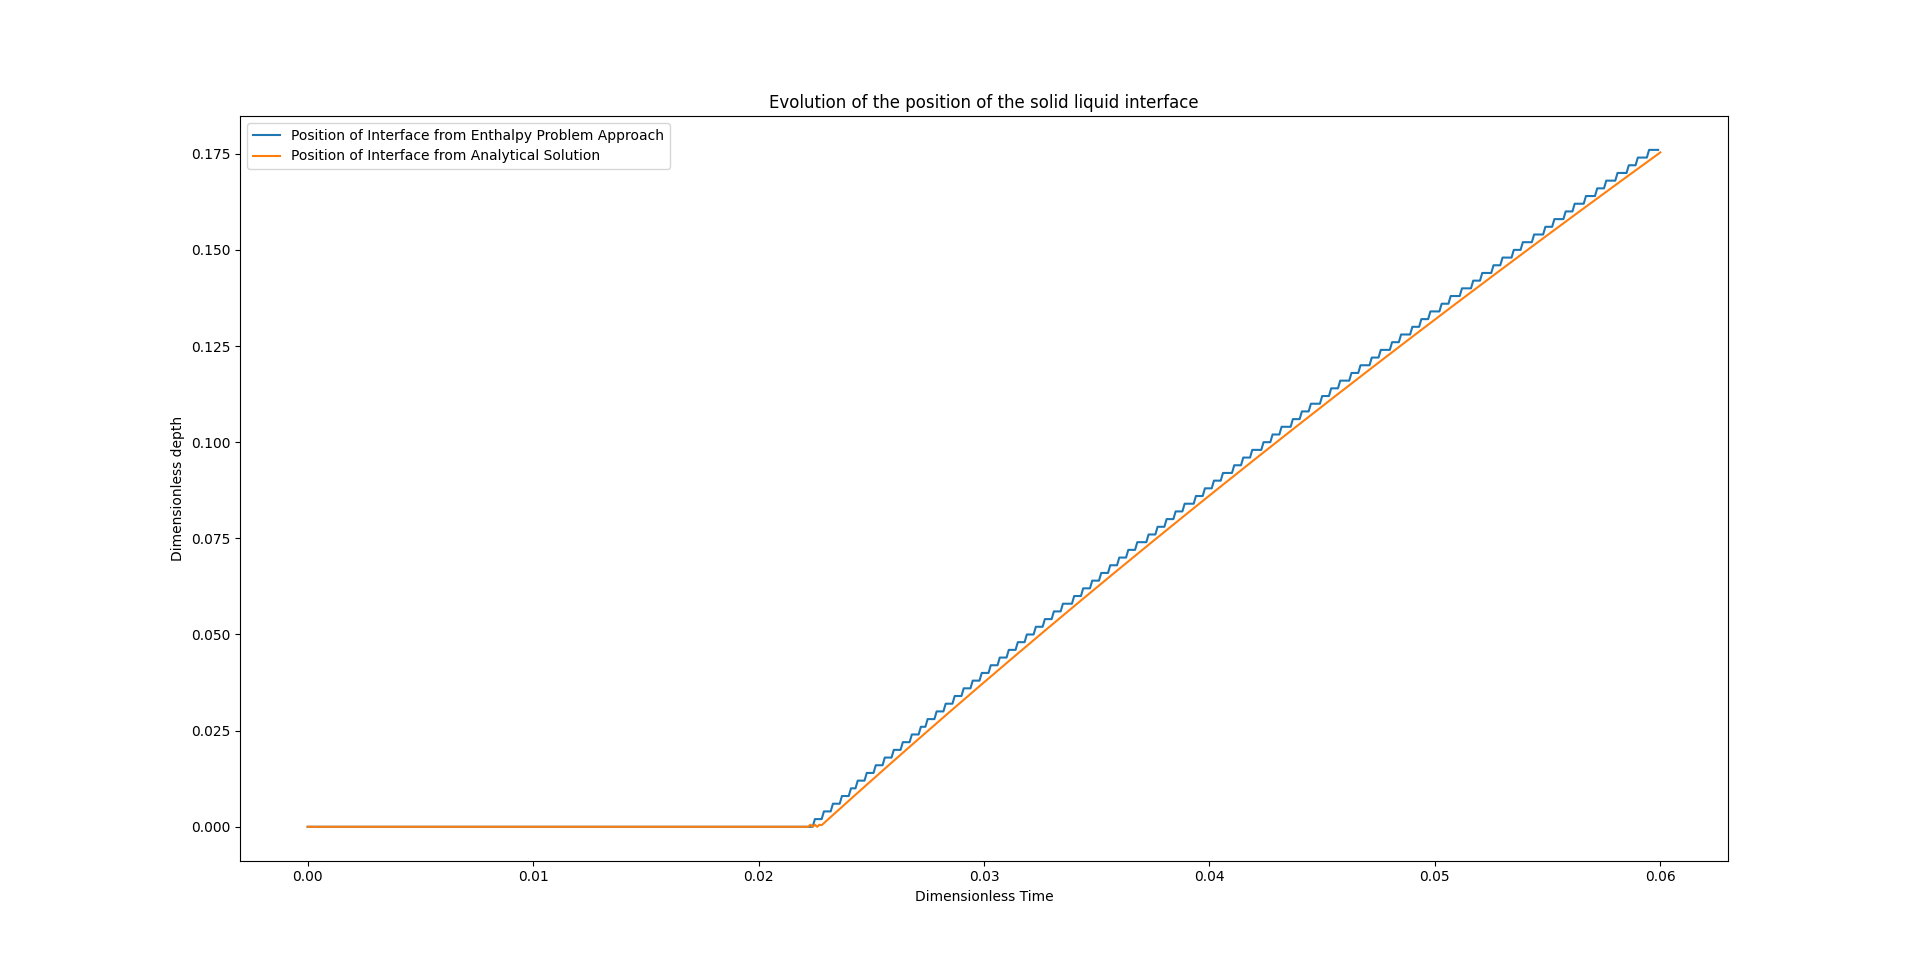
\includegraphics[width=17cm]{img/Evolution_of_the_mushy_zone_for_crystalline_material_under_301_nodes.png}
  \caption{Phase Change Boundary Evolution (Al, No Latent Heat, 301 Nodes)}
  \label{fig:phasechange}
\end{figure}

\begin{figure}[h]
  \centering
  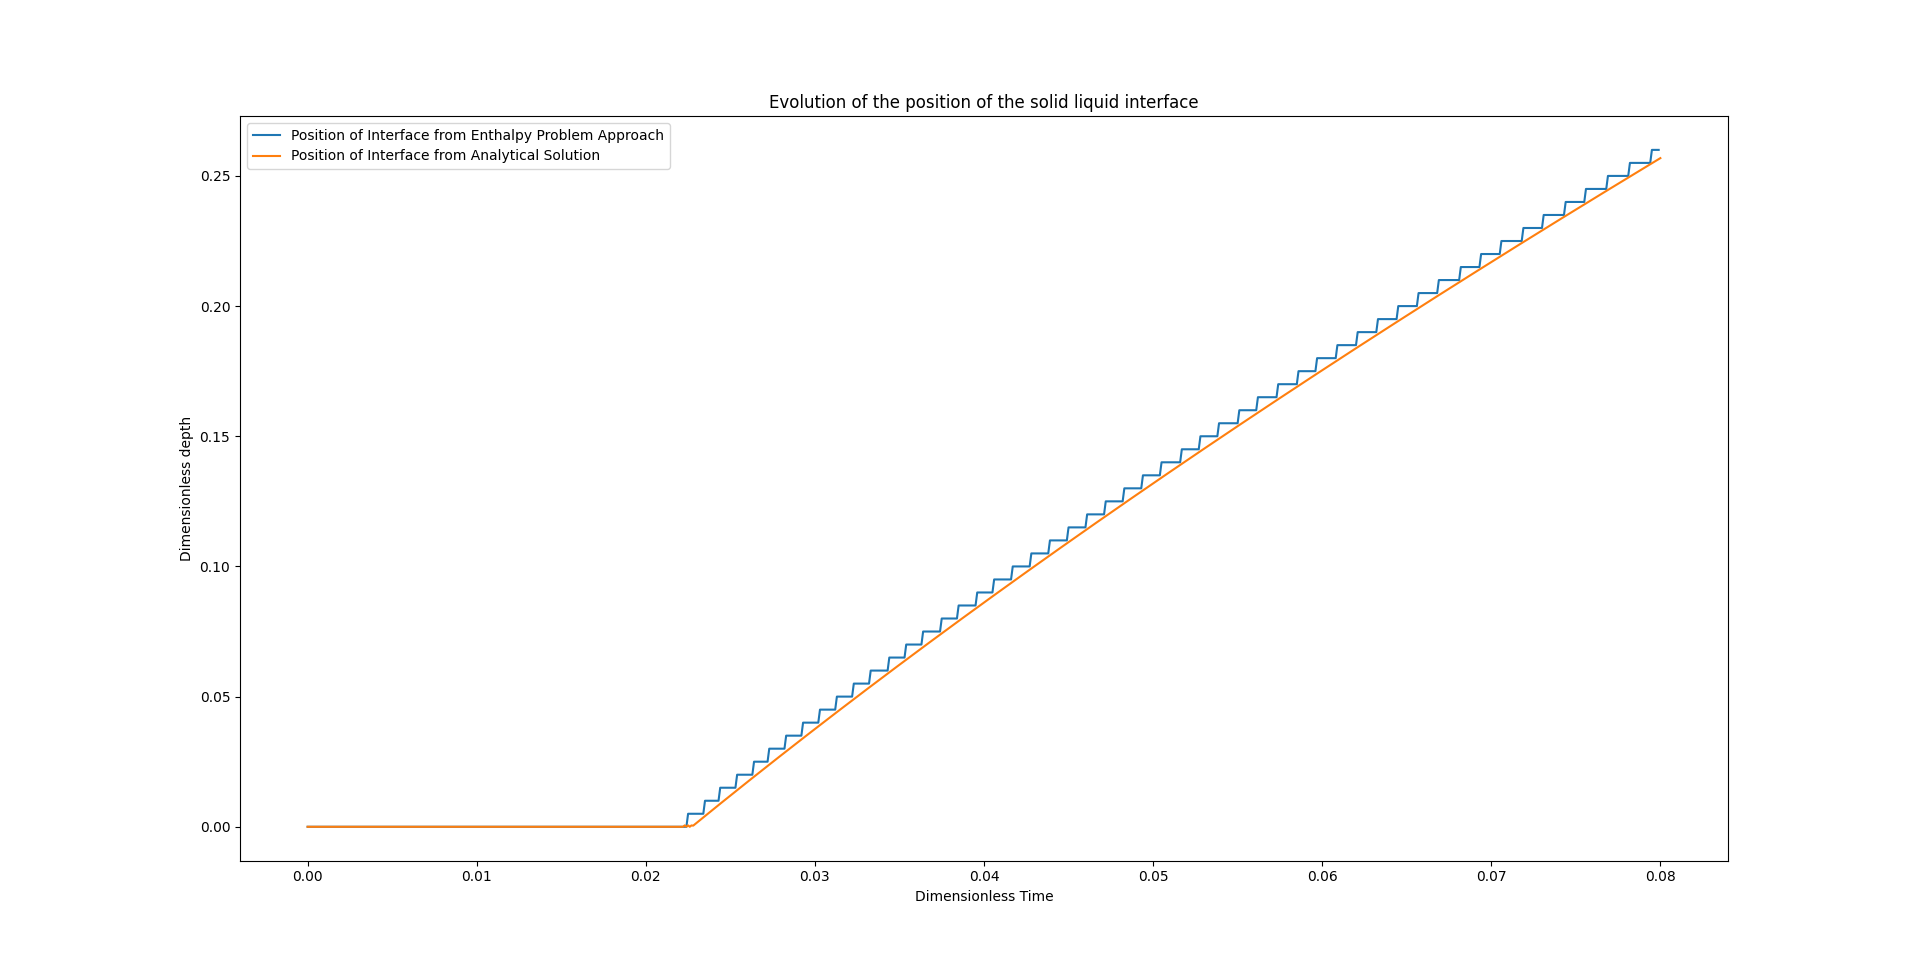
\includegraphics[width=15cm]{img/Evolution_of_the_Mushy_Zone.png}
  \caption{Phase Change Boundary Evolution (Al, No Latent Heat, 201 Nodes)}
  \label{fig:201_Nodes_phasechange}
\end{figure}

\begin{figure}[h]
  \centering
  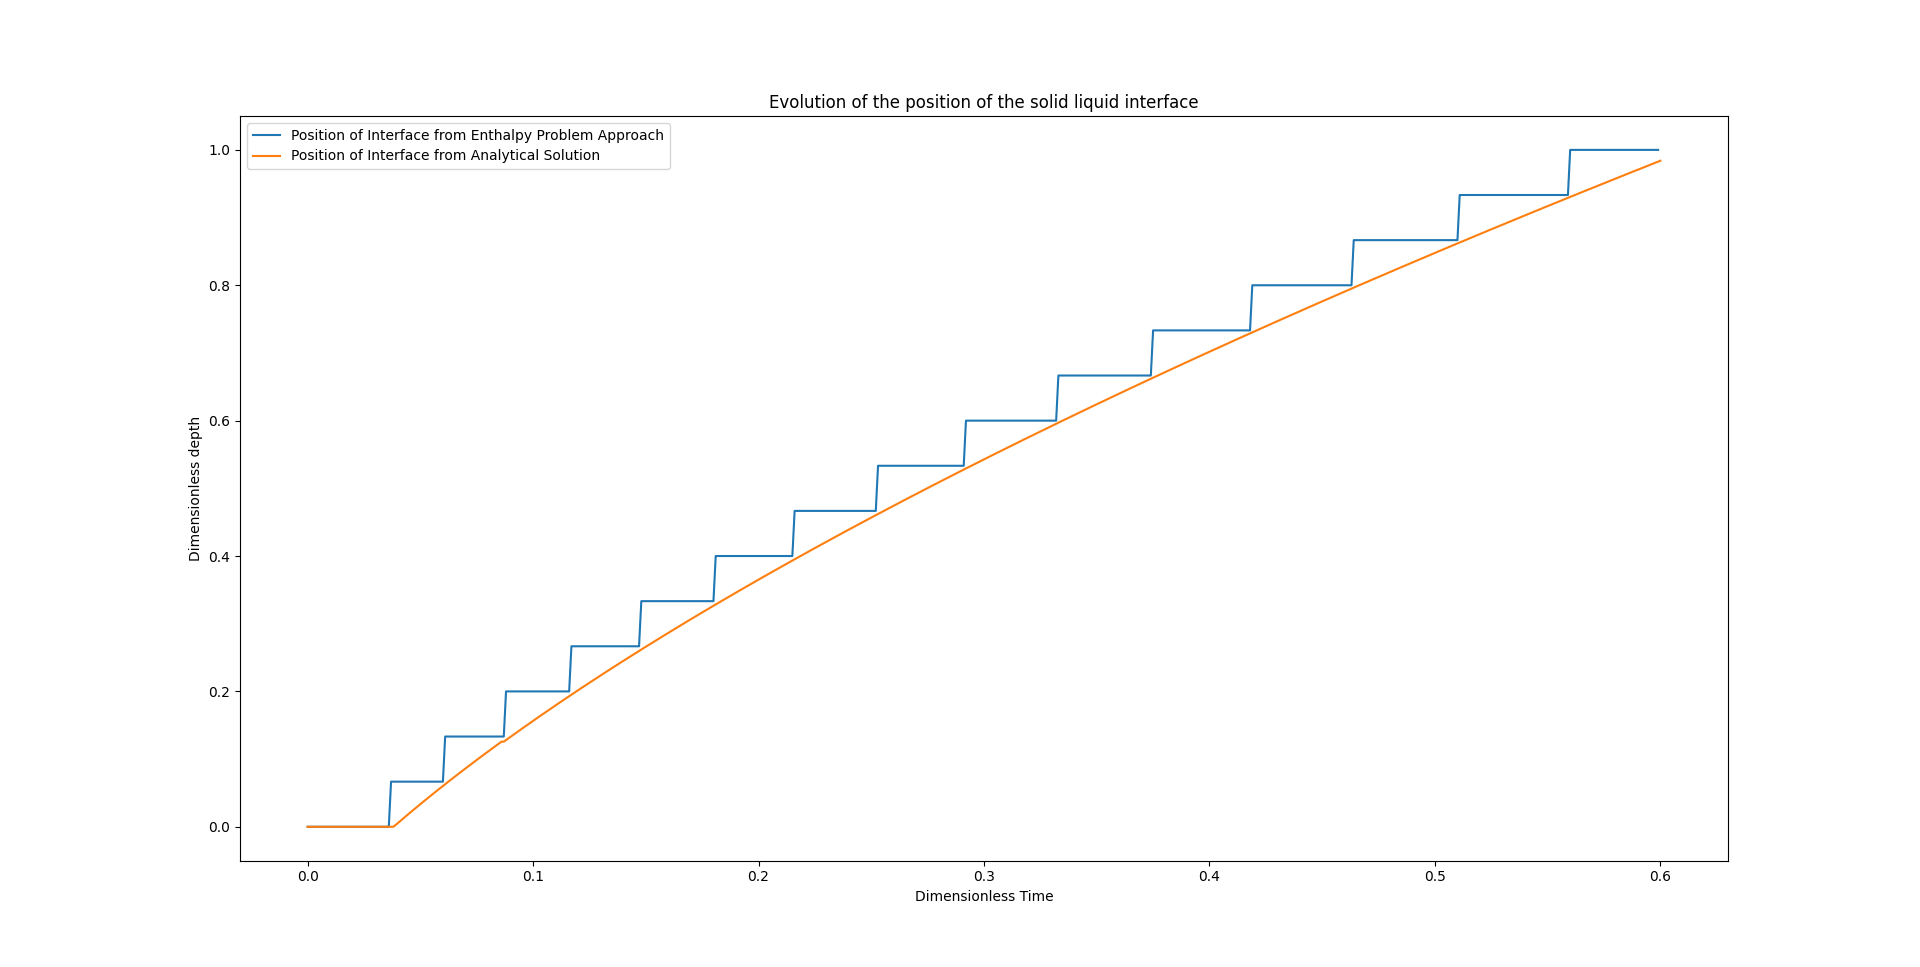
\includegraphics[width=15cm]{img/Amorphous_No_Latent_Heat_151_nodes.png}
  \caption{Phase Change Boundary Evolution (SS304L, No Latent Heat, 151 Nodes)}
  \label{fig:Amor_phasechange}
\end{figure}

\begin{figure}[h]
  \centering
  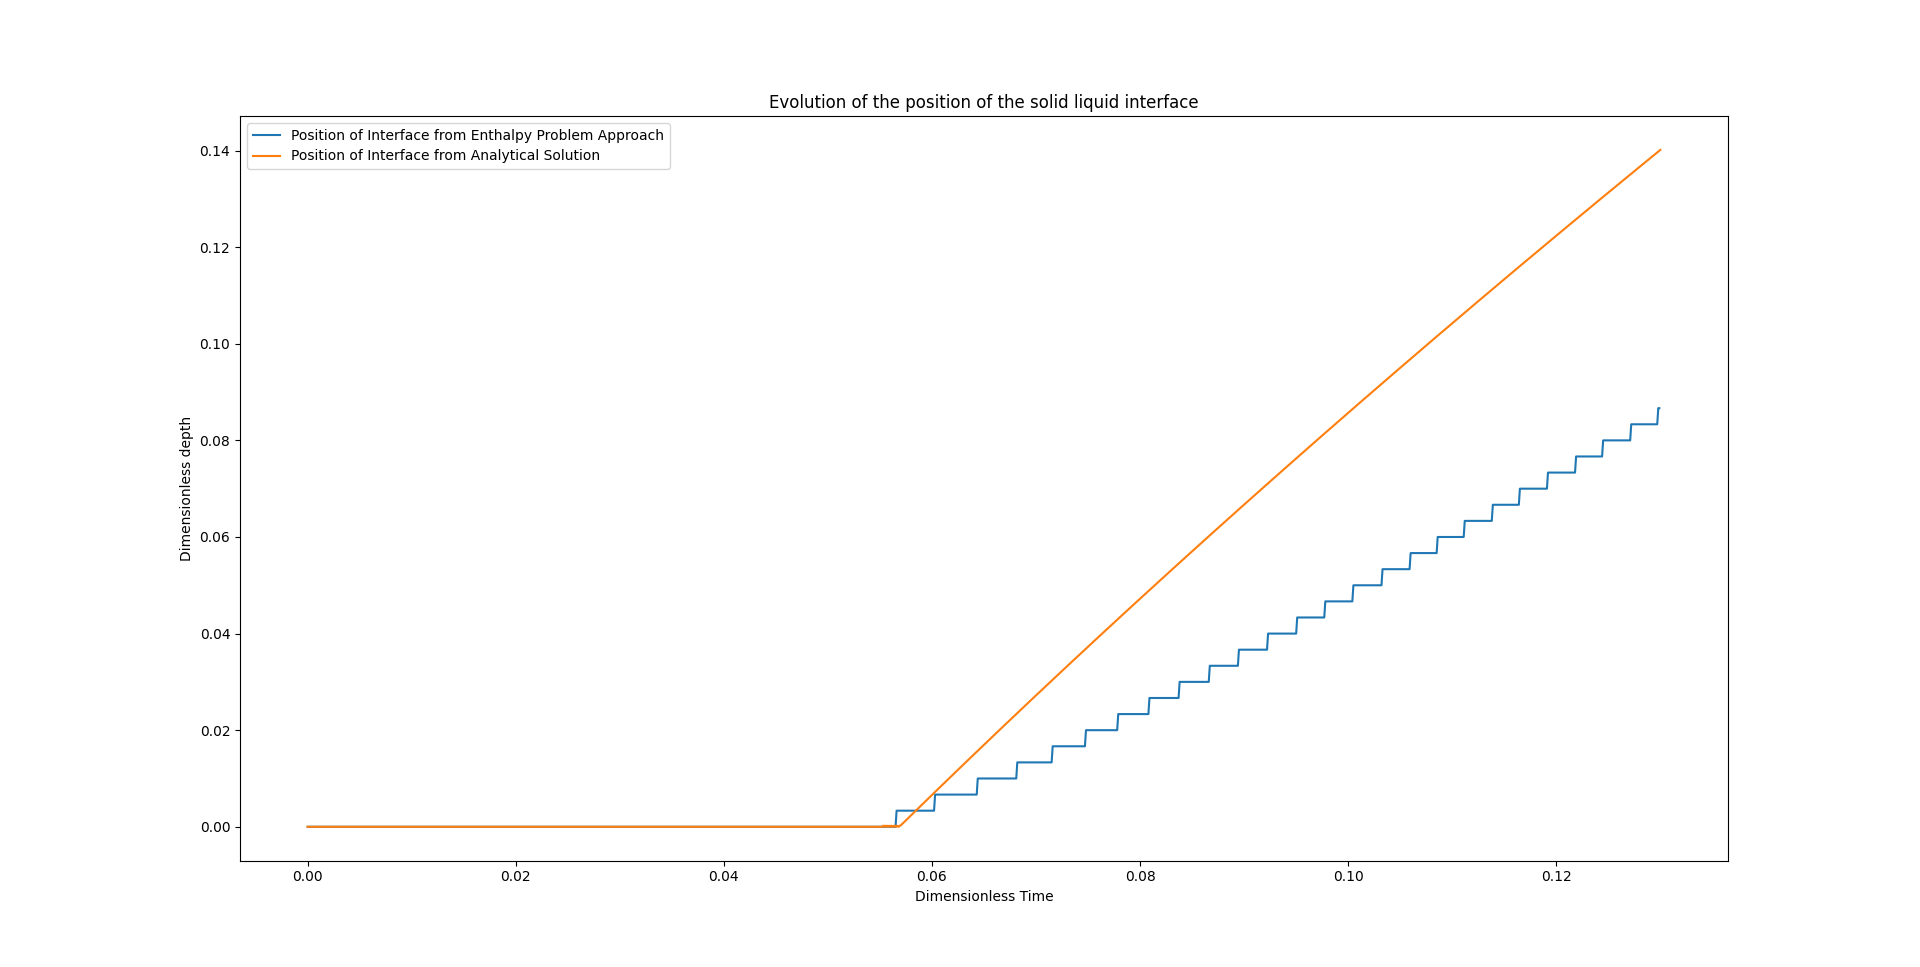
\includegraphics[width=15cm]{img/Evolution_of_mushy_zone_when_the_latent_heat_is_on.png}
  \caption{Phase Change Boundary Evolution (Al, 151 Nodes ,considering Latent Heat effects)}
  \label{fig:AL_Latenthear}
\end{figure}
\newpage
 In the in figures \ref{fig:phasechange} to \ref{fig:AL_Latenthear} we observe the staircase-like behaviour which was also observed by Ben Hills\cite{Hills_2016} in his paper. It takes time for the interface to travel through an element where tracking of the interface is impossible due to absence of nodes within the elements. The author J.C.J. Verhoeven in his paper \cite{verhoeven2003modelling} has mentioned two techniques to overcome this issue. One method is to use finer mesh (which is already done in our work) and the other is a method suggested by Tacke\cite{Tacke1985DiscretizationOT} (which we did not use in this project).\\
 We observe the impact of a finer mesh by comparing the results in Figure \ref{fig:phasechange} (301 nodes) with Figure \ref{fig:201_Nodes_phasechange} (201 nodes). The influence of considering latent heat on the interface's evolution is evident in Figure \ref{fig:AL_Enthalpy_Temperature_Latent_Heat}, while Figures \ref{fig:AL_Enthalpy_Temperature} and \ref{fig:AL_Enthalpy_Temperature_Latent_Heat} illustrate the effect of latent heat on enthalpy evolution at node 1. In our Python simulation, node 1 corresponds to the node just below the one where heat flux is applied. The figure \ref{fig:AL_Enthalpy_Temperature_Latent_Heat} and \ref{fig:SS304L_Enthalpy_Temperature_Latent_Heat} also provides a visual verification for retention of material characteristic in our material model for crystalline and amorphous material respectively. 
\begin{figure}[h]
  \centering
  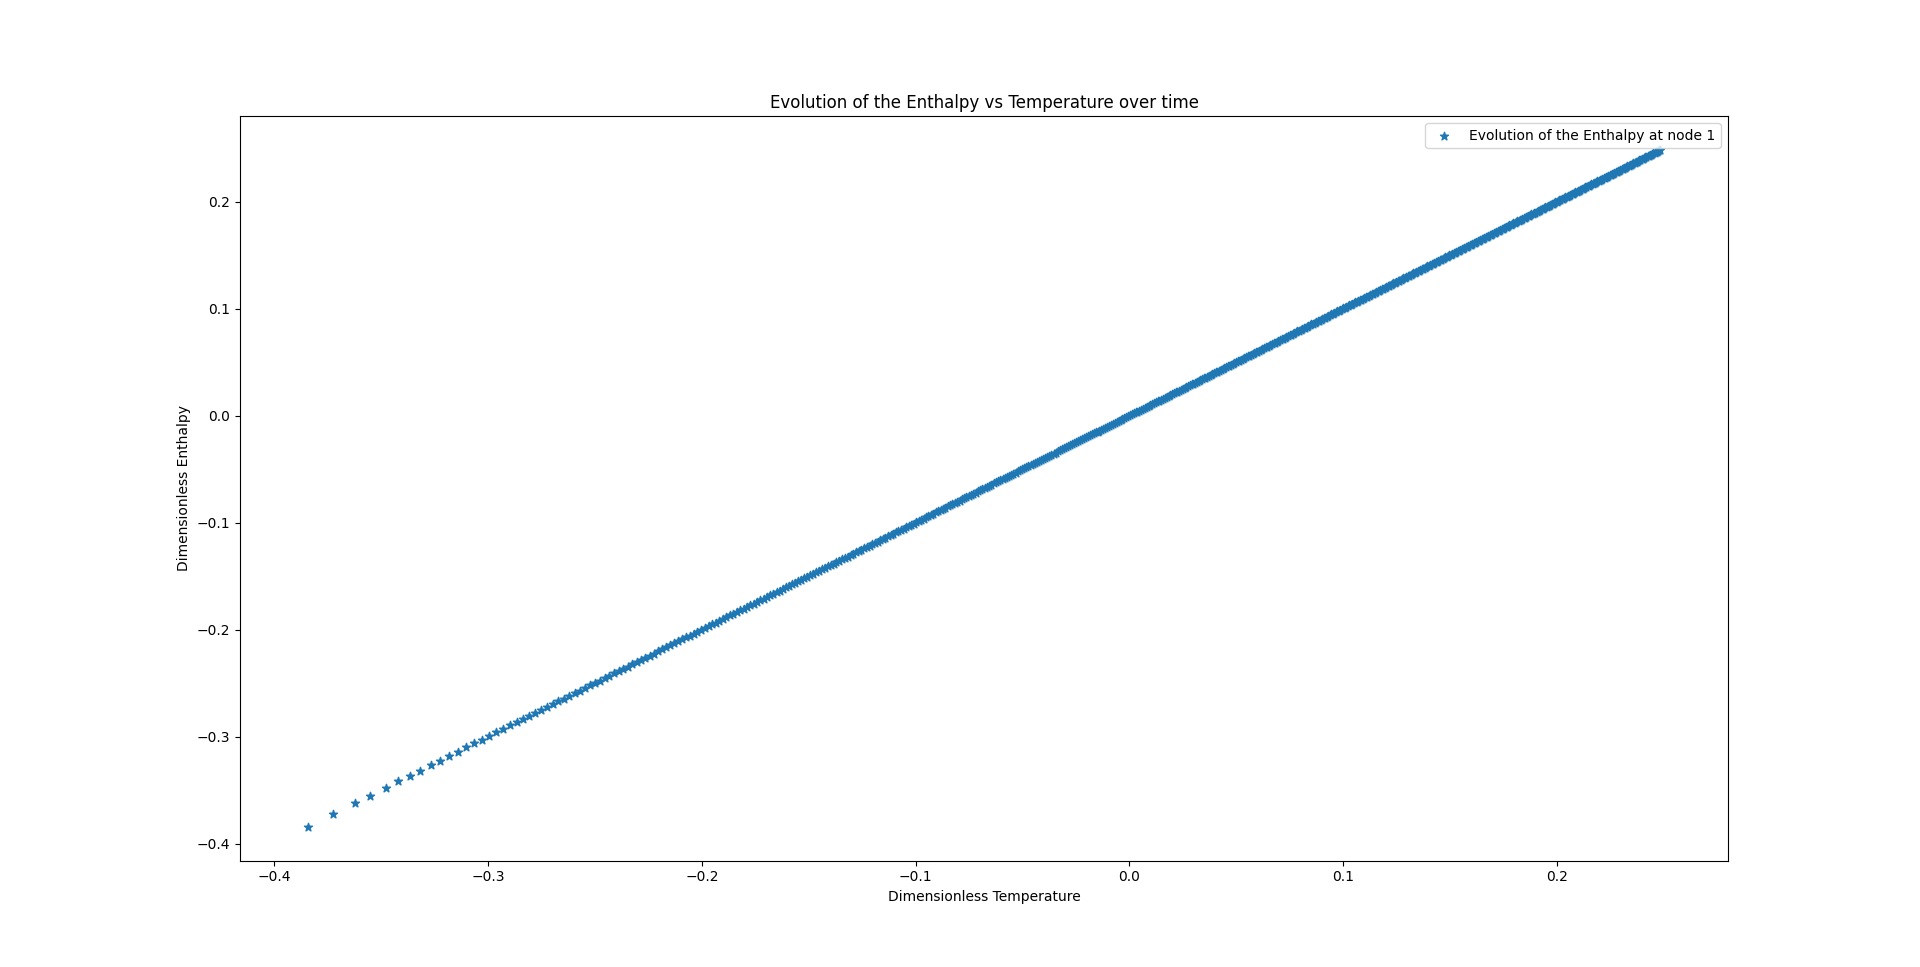
\includegraphics[width=15cm]{img/Evolution_of_Enthalpy_at_node_2_Crystalline_materials_no_latent_heat.png}
  \caption{Enthlapy vs Temperature (Al, 151 Nodes ,no Latent Heat effects considered)}
  \label{fig:AL_Enthalpy_Temperature}
\end{figure}

\begin{figure}[h]
  \centering
  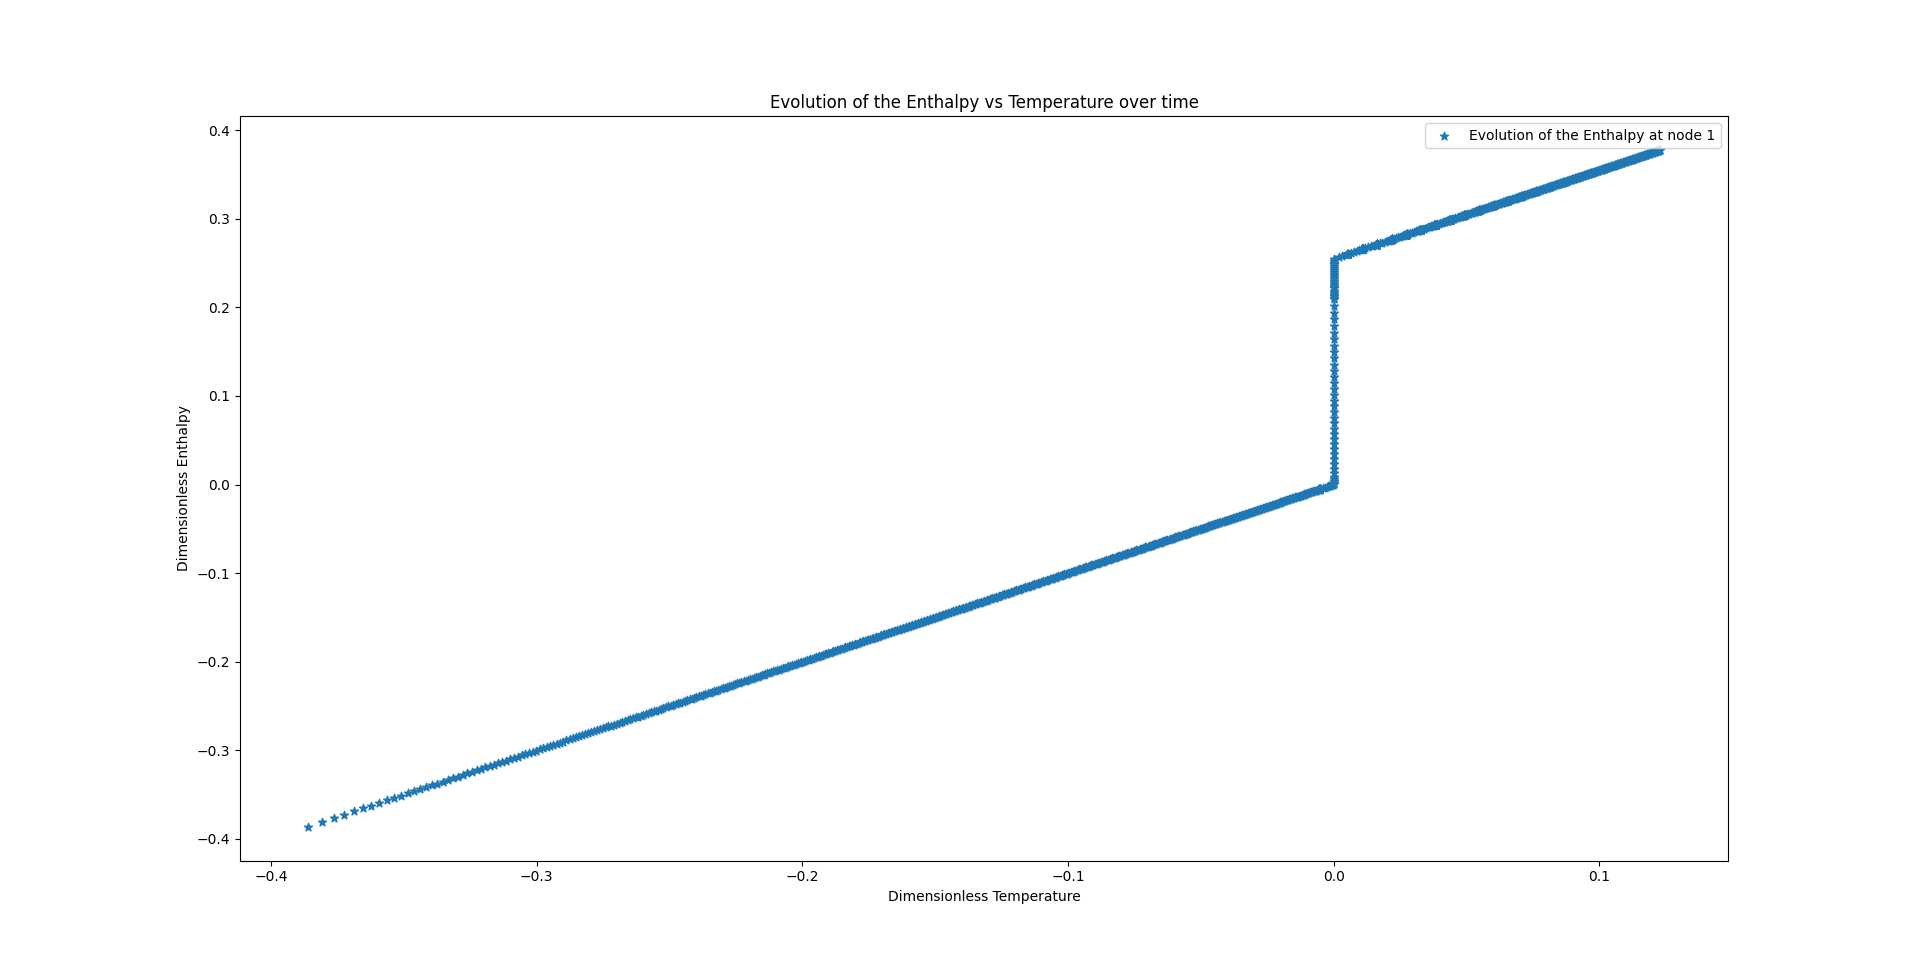
\includegraphics[width=15cm]{img/Temperature_vs_enthalpy_with_latent_heat_crystalline.png}
  \caption{Enthlapy vs Temperature (Al, 301 Nodes ,considering Latent Heat effects)}
  \label{fig:AL_Enthalpy_Temperature_Latent_Heat}
  
  \centering
  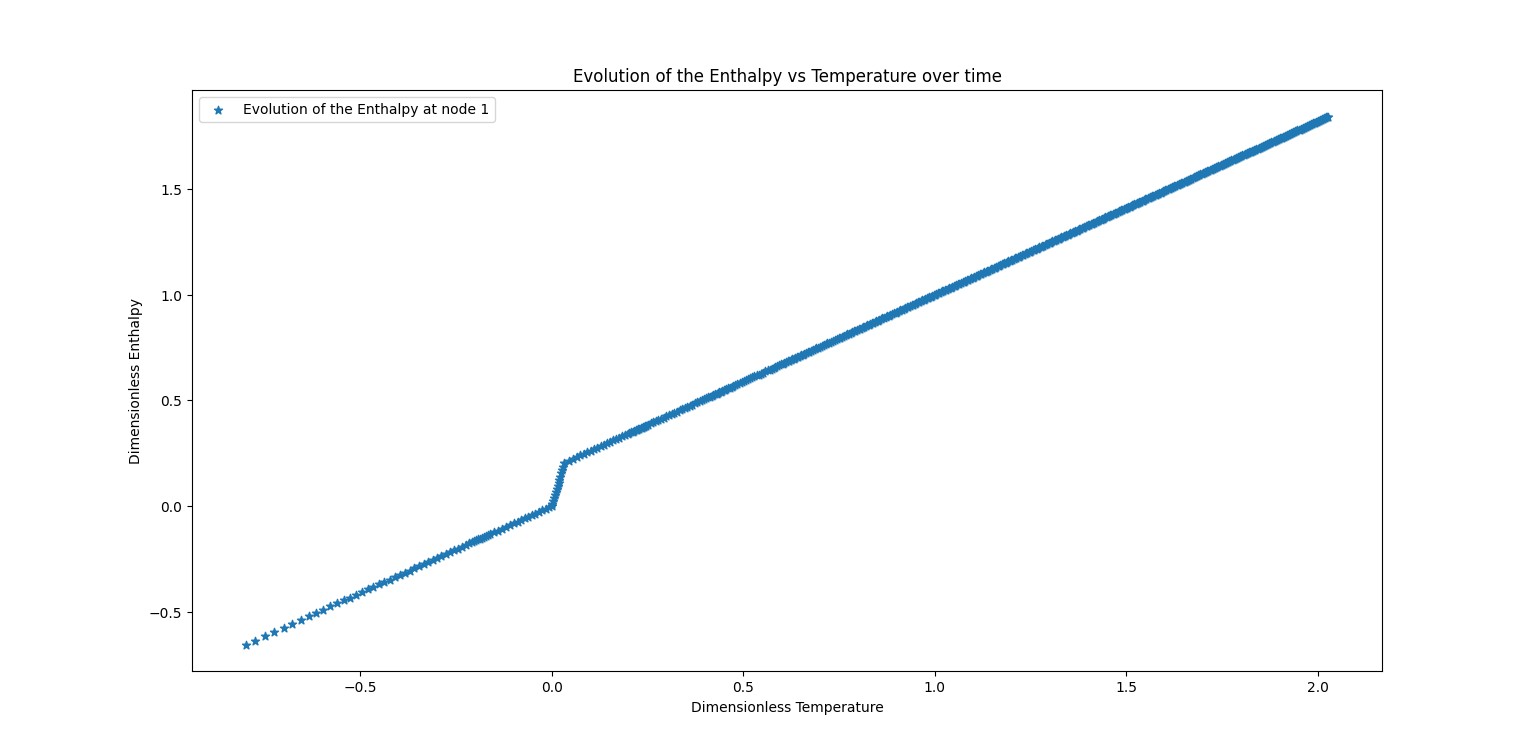
\includegraphics[width=15cm]{img/H_Tfor_amorphous.png}
  \caption{Enthlapy vs Temperature (SS304L, 151 Nodes ,considering Latent Heat effects)}
  \label{fig:SS304L_Enthalpy_Temperature_Latent_Heat}
  
\end{figure}

\begin{figure}[h]
\centering
  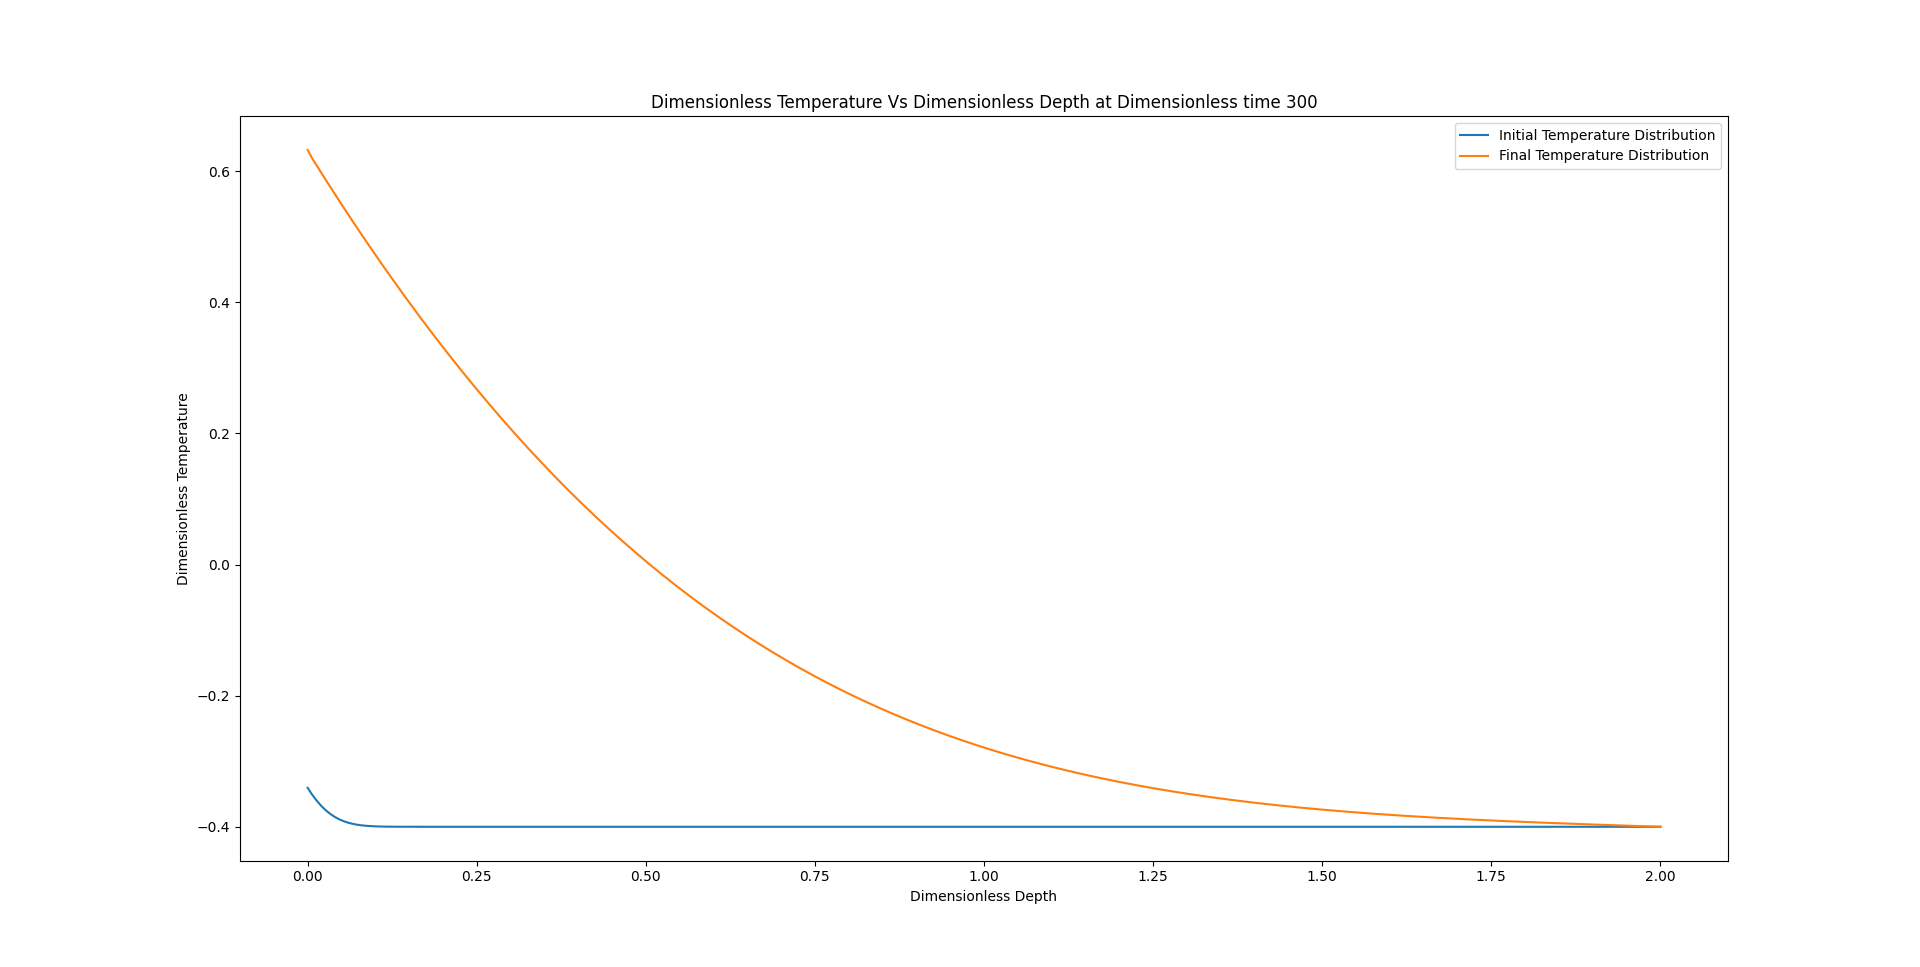
\includegraphics[width=15cm]{img/Temperature_Distribution_in_crystalline_material_Without Latent_Heat_Effects.png}
  \caption{Temperature Distribution in Al (n = 301 nodes, without considering latent heat effects)}
  \label{fig:Temperature Distribution in AL}


  \centering
  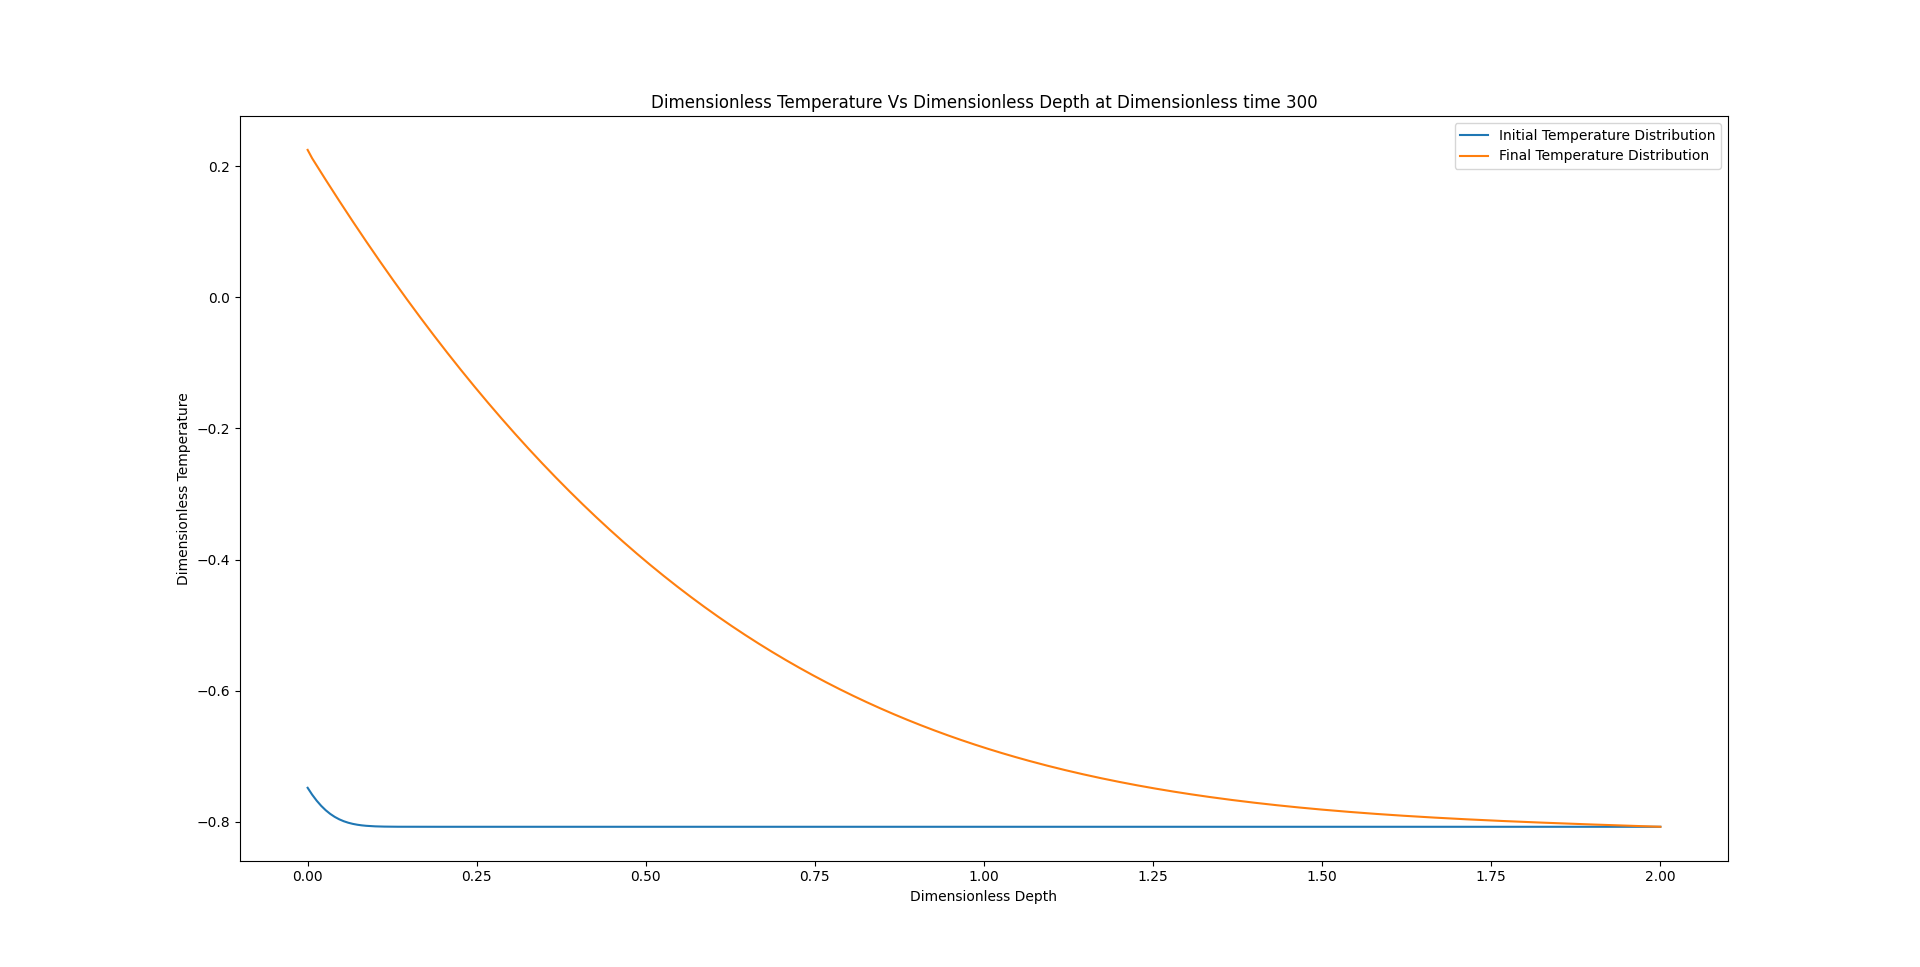
\includegraphics[width=15cm]{img/Temperature_Distribution_Amorphous.png}
  \caption{Temperature Distribution in SS304L (n = 301 nodes, without considering latent heat effects)}
  \label{fig:Temperature Distribution in SS304}
  
\end{figure}


\newpage
\section{Stefan Problem\label{sec:implaspects}}

Similar to the enthalpy problem approach, we present the results form the Stefan problem approach. For the analytical solution of the position of interface over time we employ the Euler Forward time integration scheme on the equation \ref{eq:analytical solution to the position}  and equation \ref{eq:derivativemelt_anal}. This analytical solution does not account for the latent heat. Also, due to the boundary condition \ref{eq:Stefan_specialBc}, we cannot set our latent heat equal to zero. Doing so will not allow our material to melt. Also, it is important to note that this scheme is not applicable to the amorphous material as it does not have sharp melting point. We have assumed $I = 1.5 \times 10^{10} \frac{W}{m^2}$ laser input intensity and 2 nodes in the liquid domain and 51 nodes in the solid domain for the following simulation results. The decision to employ only 2 nodes in the liquid domain was based on the initial conditions, where the liquid domain is minimal, if not negligible. The $\Delta t$ was assumed to be  0.00001.  
\begin{figure}[h]
  \centering
  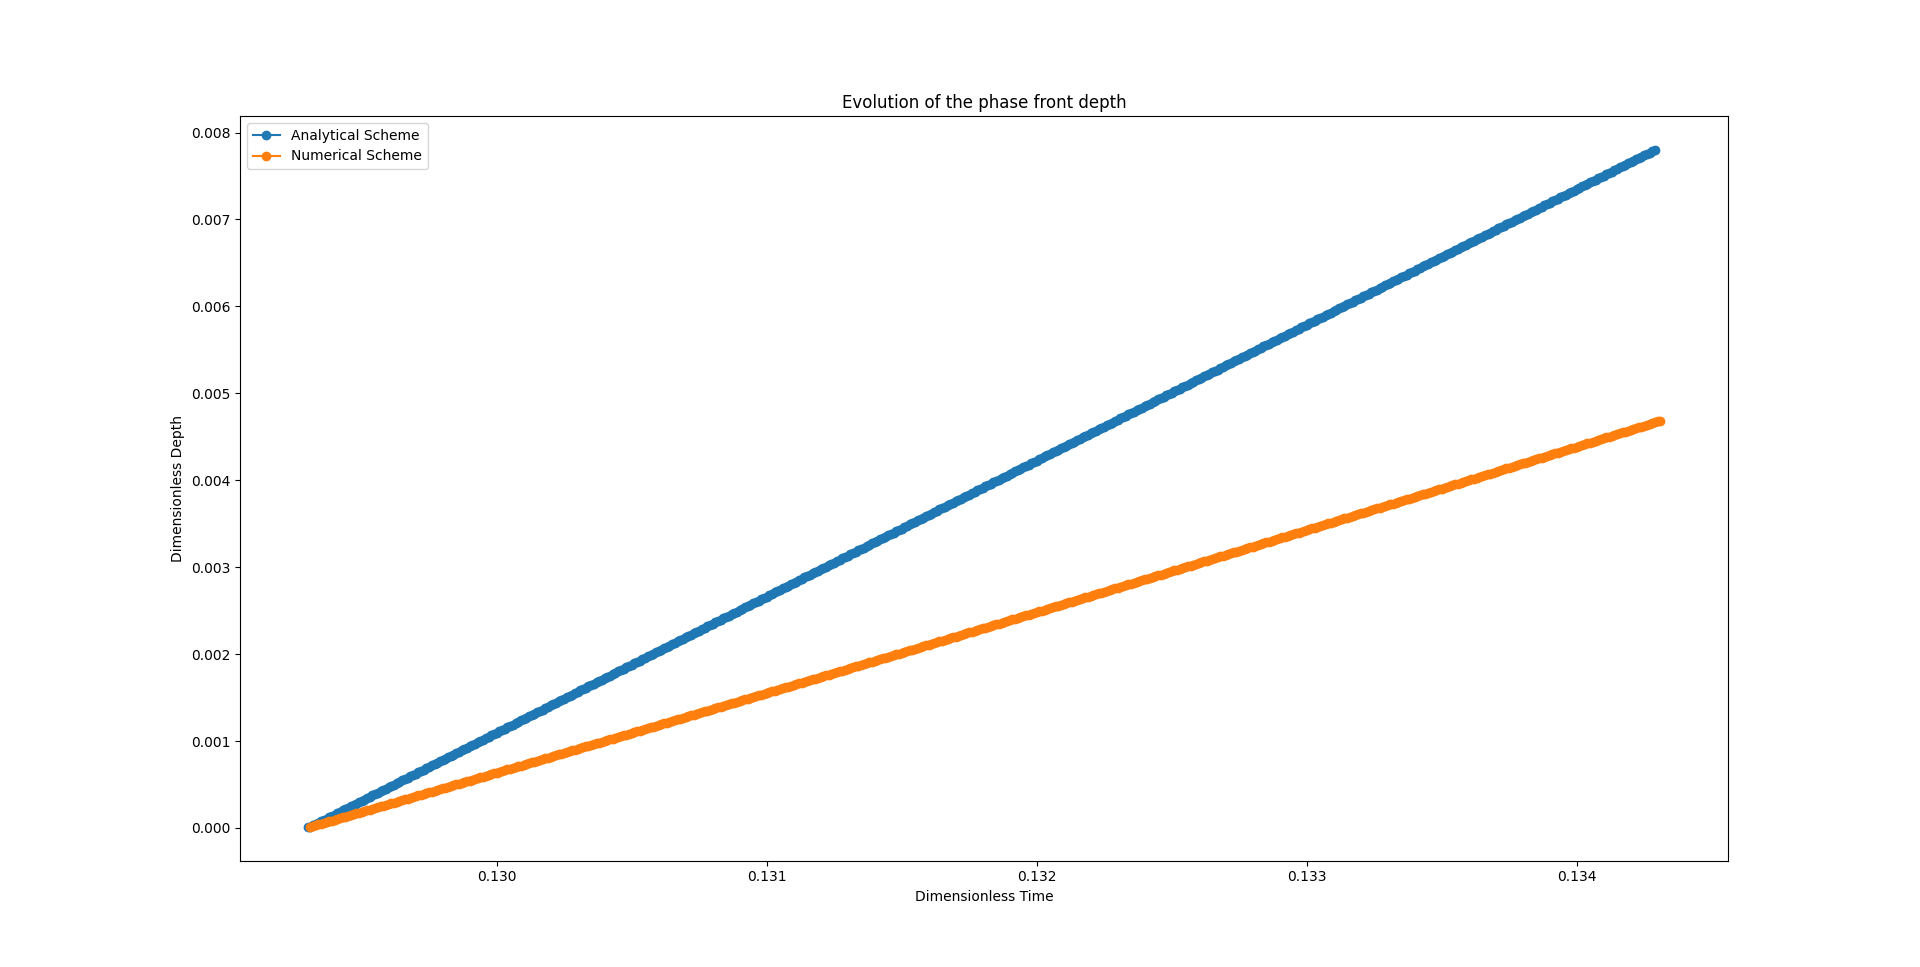
\includegraphics[width=15cm]{img/StefanMelting.png}
  \caption{Position of the phase front from numerical scheme (considering the latent heat) and analytical scheme (neglecting the latent heat effects)}
  \label{fig:Stefan melt phase front}
  \centering
  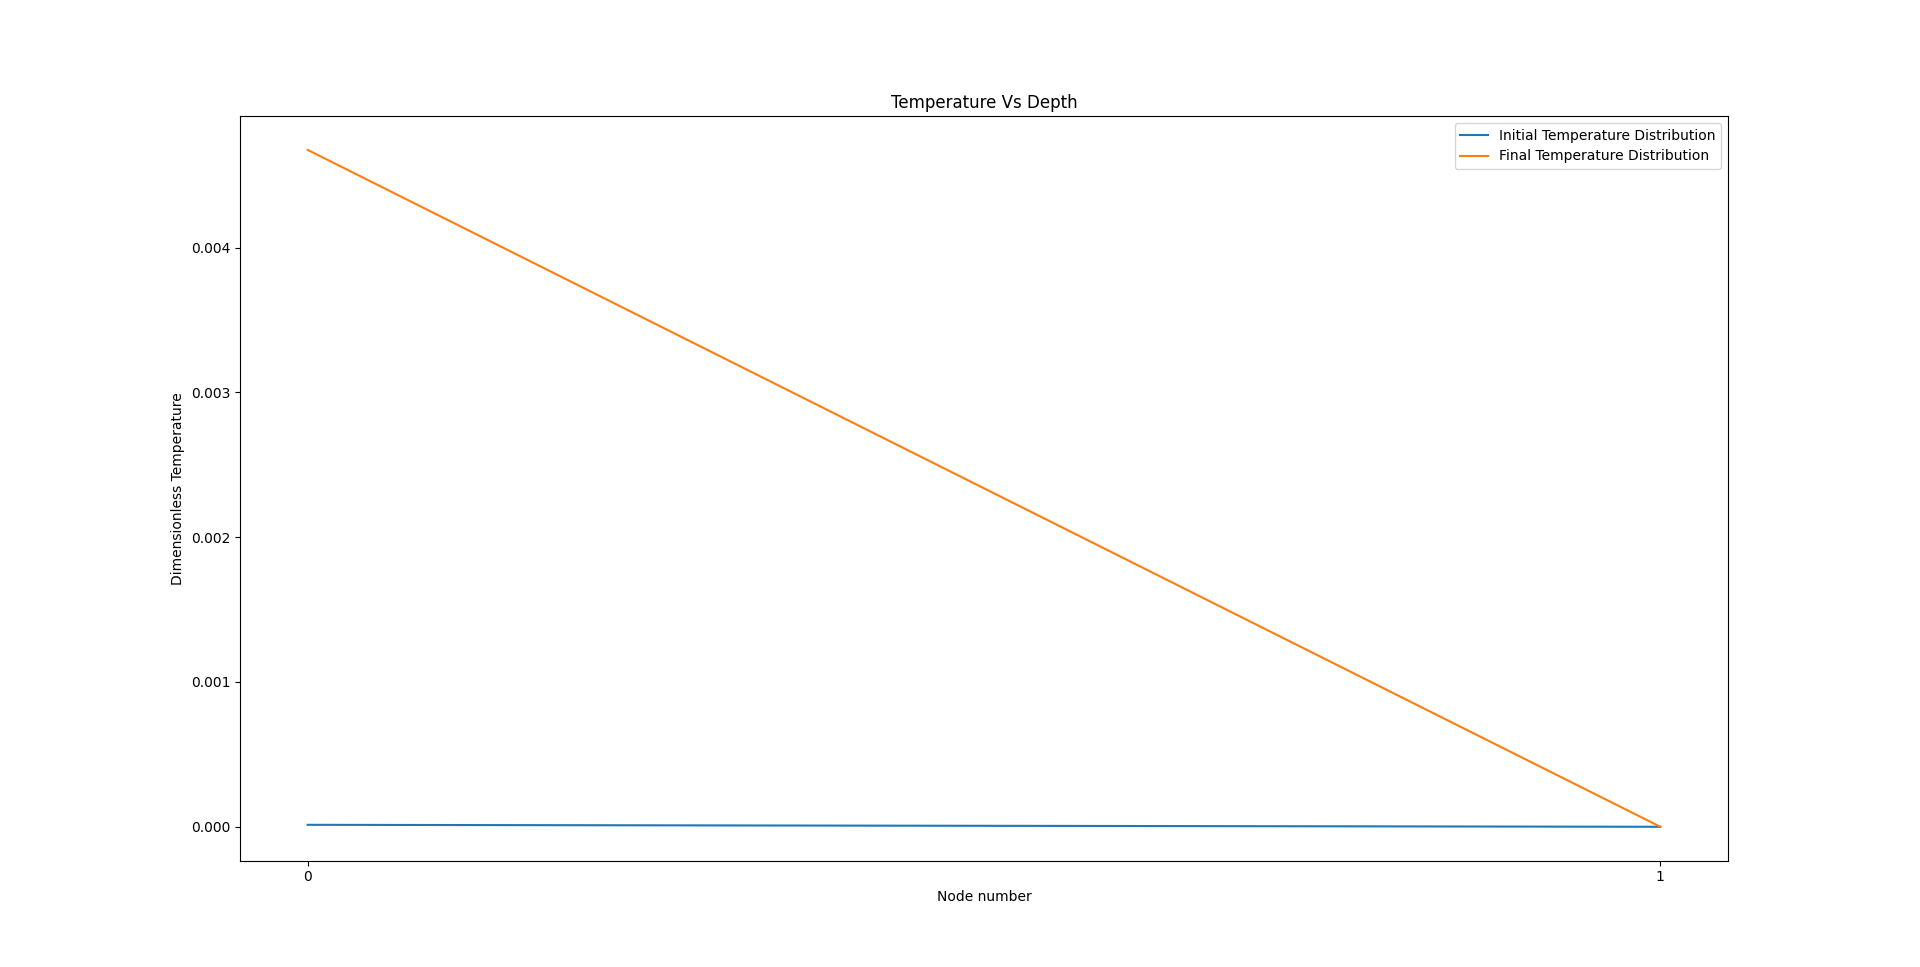
\includegraphics[width=15cm]{img/Stefan_Temp1.png}
  \caption{Temperature distribution in the liquid domain}
  \label{fig:Stefan liq temp}
  \end{figure}
  \begin{figure}[h]
  \centering
  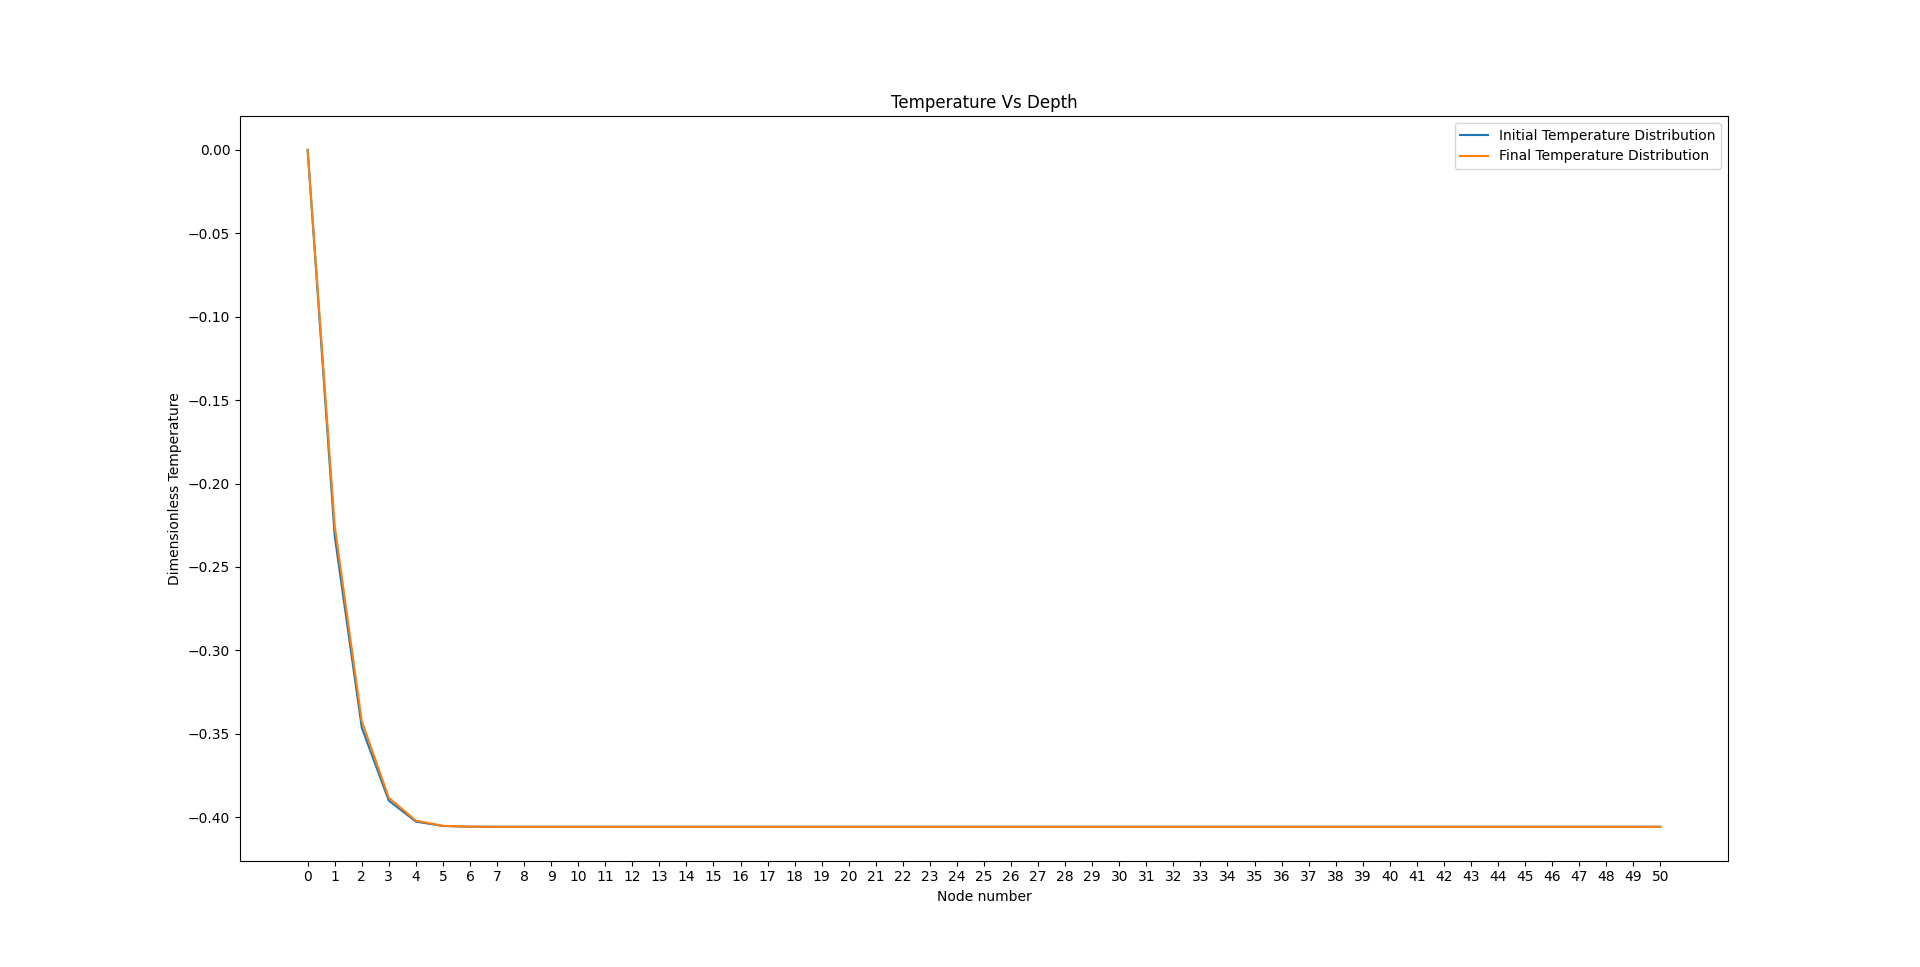
\includegraphics[width=14cm]{img/Stefan_Temperature2.png}
  \caption{Temperature distribution in the solid domain}
  \label{fig:Stefan melt front}
\end{figure}

\subsection{Enthalpy Problem 2D results}
Again we assumed a unit square. We supplied the top left corner node with the laser input. The bottom and the right edge were kept at constant ambient temperature. The results figure \ref{fig:settings for the 2D enthalpy problem} shows the simulation setup. 

\begin{figure}[h]
  \centering
  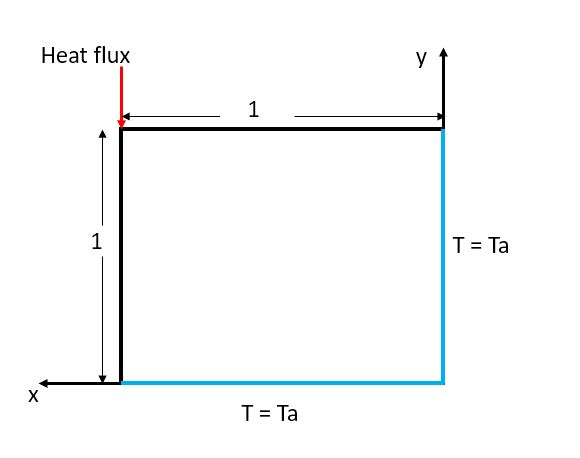
\includegraphics[width=7cm]{img/2Dsetup.png}
  \caption{Settings for the 2D Enthalpy problem}
  \label{fig:settings for the 2D enthalpy problem}
\end{figure}

\begin{figure}[h]
  \centering
  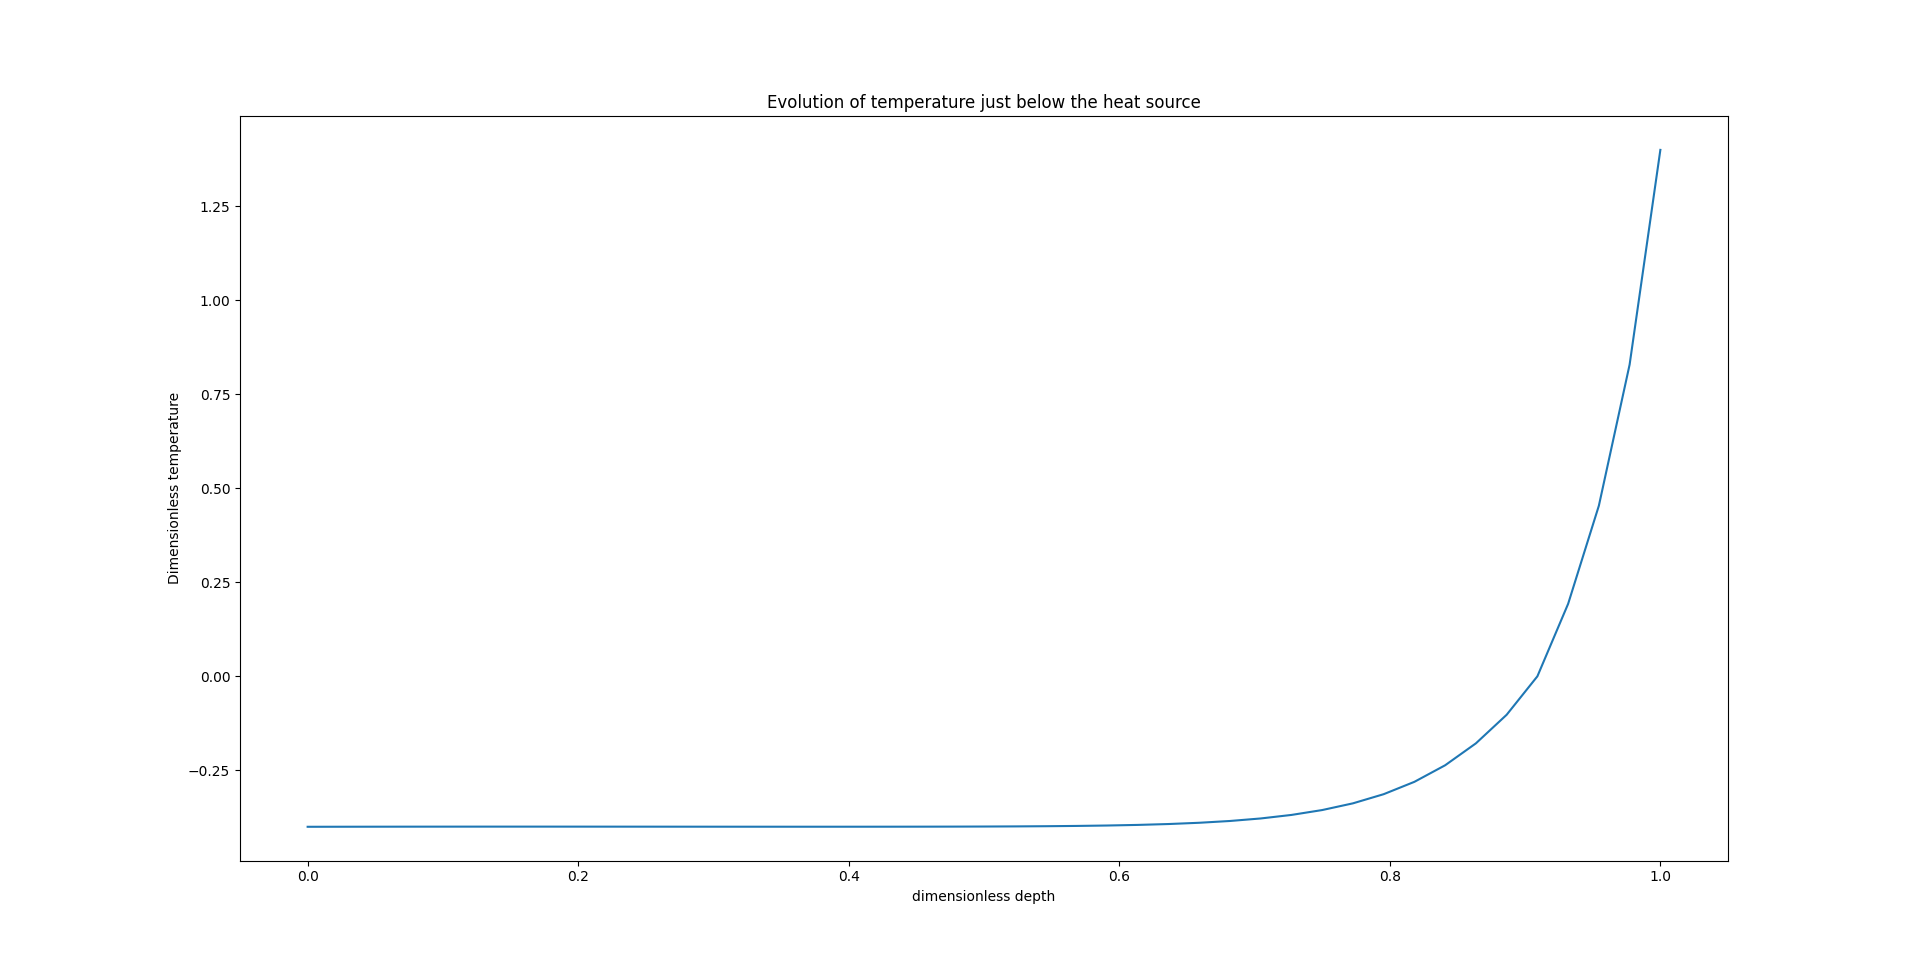
\includegraphics[width=14cm]{img/2D_Enthalpy_Temperature.png}
  \caption{Temperature evolution from the node just below the heat source}
  \label{fig:Temp just below node}
\end{figure}
The figure \ref{fig:Temp just below node} shows the evolution of the temperature over the entire simulation time.  
\begin{figure}[h]
  \centering
  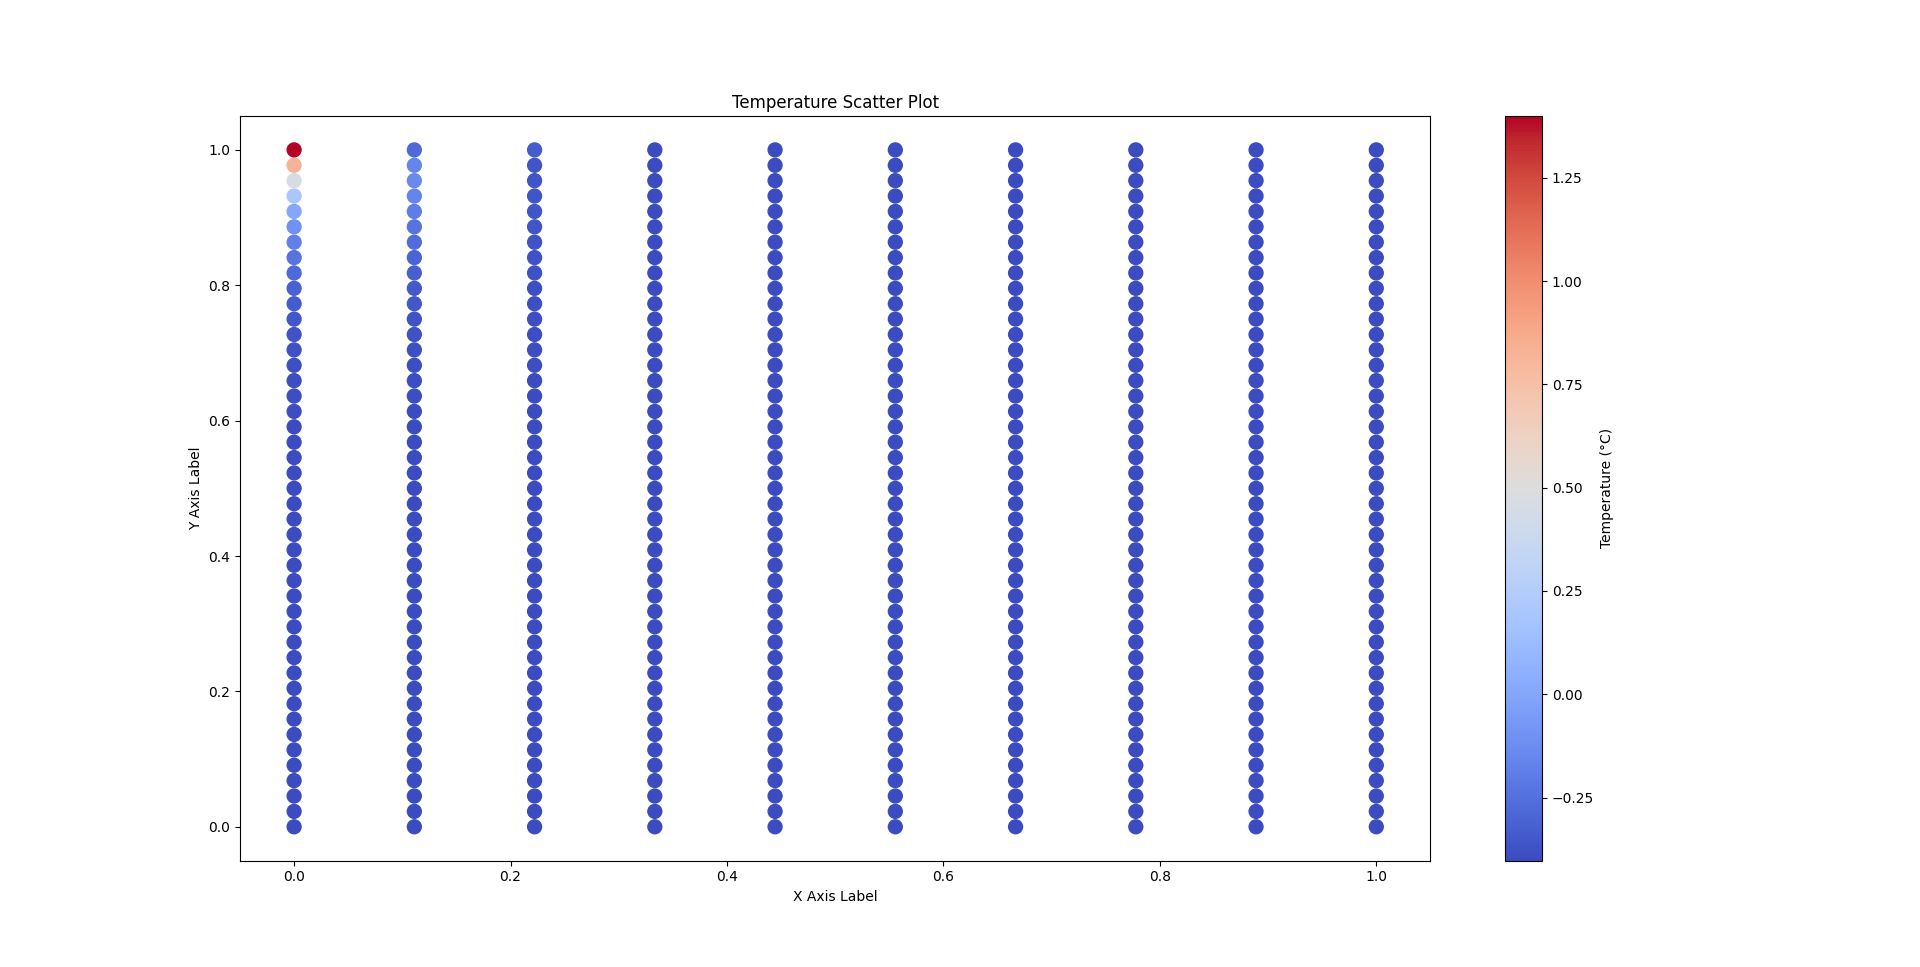
\includegraphics[width=14cm]{img/Temp_2D_Dist_Enthalpy.png}
  \caption{Temperature distribution in the matrix at end time}
  \label{fig:matrix temp end time}
\end{figure}
The figure \ref{fig:matrix temp end time} shows the temperature distribution over the entire domain at the end of simulation time. We can see that first few nodes are in the liquid regime. It is also important to note that the scheme shows convergence issues, when the temperature at node 0 goes beyond unity as it physically means that the material is evaporated. 
\newpage
\chapter{User Manual}{\label{cha:Manual}}

\section{List of files and folders}
\subsection{Enthalpy\_Approach\_1D}
\begin{enumerate}
    \item Amorphous\textunderscore inputs.py
    \item Crystalline\textunderscore inputs.py
    \item Elemental\textunderscore Subroutine.py
    \item FEA\textunderscore solve.py
    \item Initial\textunderscore Temperature\textunderscore Dist.py
    \item Material\textunderscore Subroutine.py
    \item Mesh.py
    \item postProcessor.py
    \item Processed\textunderscore inputs.py
    \item variableUpdater.py
\end{enumerate}
\subsection{Enthalpy\_Approach\_2D}
\begin{enumerate}
    \item Amorphous\textunderscore inputs.py
    \item Crystalline\textunderscore inputs.py
    \item Elemental\textunderscore Subroutine.py
    \item FEA\textunderscore solve.py
    \item Gridify.py
    \item Initial\textunderscore Temperature\textunderscore Dist.py
    \item Material\textunderscore Subroutine.py
    \item Processed\textunderscore inputs.py
    \item variableUpdater.py
\end{enumerate}
\subsection{Heat\textunderscore Transfer\textunderscore Verification}
Along with the above mentioned files the Heat\textunderscore Transfer\textunderscore Verification has one more additional file Heat\textunderscore Transfer\textunderscore Verification.py. The file Initial\textunderscore Temperature\textunderscore Dist.py is changed in this folder. Remaining all the files are same. 
\subsection{Testing}
\begin{enumerate}
    \item Amorphous\textunderscore inputs.py
    \item Crystalline\textunderscore inputs.py
    \item Gridify.py
    \item Mesh.py
    \item Mesh\textunderscore Test.py
    \item Processed\textunderscore inputs.py
    \item Processed\textunderscore inputsA.py
    \item slope\textunderscore matrix.py
    \item Slope\textunderscore MatrixA.py
    \item Test\textunderscore Amorphous.py
    \item Test\textunderscore Crystalline.py
    \item Test\textunderscore Mesh\textunderscore 2D.py
\end{enumerate}
The Gridify.py is the 2D mesh file, Slope\textunderscore MatrixA.py and slope\textunderscore matrix.py are part of Material\textunderscore Subroutine.py. All the other files such as Processed\textunderscore inputs.py and Processed\textunderscore inputsA.py are same just the material selected is different.  
\subsection{Stefan\_ Approach}
\begin{enumerate}
    \item Crystalline\textunderscore inputs.py
    \item Elemental\textunderscore Subroutine.py
    \item FEA\textunderscore solve.py
    \item Initial\textunderscore Conditions.py
    \item postProcessor.py
    \item Processed\textunderscore inputs.py
    \item variableUpdater.py
\end{enumerate}
\section{Libraries used}
The libraries we used in programming the simulation is shown in table \ref{tab:softwares used}. \\
\begin{table}[h]
    \centering
    \begin{tabular}{|c|c|} \hline 
         \textbf{Library / Software}& \textbf{Version}\\ \hline 
 Python &3.11.2\\ \hline 
         Numpy& 1.24.1\\ \hline 
         math& 3.5\\ \hline 
         matplotlib& 3.6.3\\ \hline
 Time&3.11.2 (inbuilt)\\\hline
    \end{tabular}
    \caption{Libraries used and their versions}
    \label{tab:softwares used}
\end{table}
\noindent The installation of the libraries mentioned in table \ref{tab:softwares used} can be done as follows:-\\
Installing the numpy.\\
\indent \indent \$ pip install numpy\\
Installing the math.\\
\indent \indent \$ pip install math\\
Installing the numpy.\\
\indent \indent \$ pip install matplotlib\\
\section{Running the program}
\begin{enumerate}
    \item To begin, please navigate to the folder that contains the files related to the simulation you desire to run.
    \item   The files 'Amorphous\textunderscore inputs.py' and 'Crystalline\textunderscore inputs.py' contains the inputs which can be edited for user defined inputs.
    \item Next, select the type of material in the 'Processed\textunderscore inputs.py' by setting the mat\textunderscore type = 1 for the crystalline material and 2 for the amorphous material for the enthalpy problem approach. Note for Stefan problem approach this variable is always = 1.
    \item    Afterward the simulation can be run using the command line with the command python .\textbackslash FEA\textunderscore solve.py for standard Windows operating system.
    \item Finally, the results will be displayed as graphs and on the command line as well.
\end{enumerate}
\newpage
\chapter{Computation time study}{\label{cha:Computational Study time}}
The 'time' module is built into the Python interpreter, and we have utilized this module in our program to measure the time required for the execution of each module. The modules and their respective execution times are presented in Table \ref{tab:computational time study}.\\
\begin{table}[h]
    \centering
    \begin{tabular}{|c|c|} \hline  
         \textbf{Library}& \textbf{Time} (in s)\\ \hline  
         Mesh& 0\\ \hline  
 Gridify&0.01\\ \hline 
         Initial\textunderscore Temperature\textunderscore Dist& 0\\ \hline  
         variableUpdater& 0\\ \hline  
         Elemental\textunderscore Subroutine& 0.491\\ \hline  
         FEA\textunderscore solve& 16.3031\\ \hline  
         postProcessor& 9.6406\\ \hline 
    \end{tabular}
    \caption{Computation time study}
    \label{tab:computational time study}
\end{table}
It can be observed that the solver requires the most time to execute. In the previous versions of the program, where the assembly was done using the assignment matrix, the time required was quite large. Introduction of mesh list removed the need of assignment matrix. Hence, an improvement in the computational time was observed. Further, the computational time can be reduced by utilizing the 'scipy' package in python which includes a sparse matrix solver. This solver is considerably more efficient than computing the inverse of the stiffness matrix, which is computationally expensive. Additionally, the assembly is now done in a separate function, which allows parallelization of the execution.